%%%  Ukázkový text a dokumentace stylu pro text závěrečné (bakalářské a diplomové) práce na KI PřF UP v Olomouci
%%%  Copyright (C) 2026 Jesse Sadowý, <jesse.sadowy23@gmail.com>
%%%  Copyright (C) 2026 Jan Konečný, <jan.konecny@upol.cz>


%%  Pro získání PDF souboru dokumentu je třeba tento zdrojový text v
%%  LaTeXu přeložit (dvakrát) programem pdfLaTeX.

%%  V případě použití programu BibLaTeX pro tvorbu seznamu literatury
%%  je poté ještě třeba spustit program Biber s parametrem jméno
%%  souboru zdrojového textu bez přípony a následně opět (dvakrát)
%%  přeložit zdrojový text programem pdfLaTeX.

%%  Postup získání Postscriptového souboru je popsán v dokumentaci.


%%  Třída dokumentu implementující styl pro závěrečnou práci. Vybrané
%%  nepovinné parametry (ostatní v dokumentaci):

%%  'master' pro sazbu diplomové práce, jinak se sází bakalářská práce

%%  'program=kód' pro Váš studijní program/obor (specializaci), kódy
%%  pro diplomovou práci 'infoi' pro Informatiku (Obecná informatika),
%%  'infui' pro Informatiku (Umělá inteligence), 'ainfpst' pro
%%  Aplikovanou informatiku (Počítačové systémy a technologie), 'uinf'
%%  pro Učitelství informatiky pro střední školy, 'binf' pro
%%  Bioinformatiku, 'inf' pro Informatiku (bez specializací) a 'ainf'
%%  pro Aplikovanou informatiku (bez specializací), jinak je výchozí
%%  ainfvs pro Aplikovanou informatiku (Vývoj software), a pro
%%  bakalářskou práci 'infoi' pro Informatiku (Obecná informatika),
%%  'itp' pro Informační technologie v prezenční formě, 'itk' pro
%%  Informační technologie v kombinované formě, 'infv' pro Informatiku
%%  pro vzdělávání, 'binf' pro Bioinfomatiku, 'inf' pro Informatiku
%%  (bez specializací), 'ainfp' pro Aplikovanou informatiku (bez
%%  specializací) v prezenční formě, 'ainfk' pro Aplikovanou
%%  informatiku (bez specializací) v kombinované formě, jinak je
%%  výchozí infpvs pro Informatiku (Programování a vývoj software)

%%  'printversion' pro sazbu verze pro tisk (nebarevné logo a odkazy,
%%  odkazy s uvedením adresy za odkazem, ne odkazy do rejstříku),
%%  jinak verze pro prohlížeč

%%  'biblatex' pro zapnutí podpory pro sazbu bibliografie pomocí
%%  BibLaTeXu, jinak je výchozí sazba v prostředí thebibliography

%%  'language=jazyk' pro jazyk práce, jazyky english pro anglický,
%%  slovak pro slovenský, jinak je výchozí czech pro český

%%  'font=sans' pro bezpatkový font (Iwona Light), jinak je výchozí
%%  serif pro patkový (Latin Modern)

%%  'figures, tables, theorems a sourcecodes' pro sazbu seznamu
%%  obrázků, tabulek, vět a zdrojových kódů, jinak při =false se
%%  nesází (u theorems a sourcecodes výchozí)

\documentclass[
%  master,
   program=itk,
%  printversion,
   biblatex,
%  language=english,
%  font=sans,
   figures=true,
   tables=true,
%  theorems,
%  sourcecodes,
   glossaries,
   index
]{kidiplom}

%% Informace pro úvodní strany. V jazyku práce (pokud není v komentáři
%% uvedeno česky) a anglicky. Uveďte všechny, u kterých není v
%% komentáři uvedeno, že jsou volitelné. Při neuvedení se použijí
%% výchozí texty. Text pro jiný než nastavený jazyk práce (nepovinným
%% parametrem language makra \documentclass, výchozí český) se zadává
%% použitím makra s uvedením jazyka jako nepovinného parametru.

%% Název práce, česky a anglicky. Měl by se vysázet na jeden řádek.
\title{Procedurální generování dungeonů ve 2D hrách}
\title[english]{Procedural Generation of Dungeons in 2D Games}

%% Volitelný podnázev práce, česky a anglicky. Měl by se vysázet na
%% jeden řádek. Výchozí je prázdný.
\subtitle{Implementace a~srovnání algoritmů v~herním enginu Godot}
\subtitle[english]{Implementation and Comparison of Algorithms in Godot Game Engine}

%% Jméno autora práce. Makro nemá nepovinný parametr pro uvedení
%% jazyka.
\author{Jesse Sadowý}

%% Jméno vedoucího práce (včetně titulů). Makro nemá nepovinný
%% parametr pro uvedení jazyka.
\supervisor{doc. RNDr. Jan Konečný, Ph.D.}

%% Volitelný rok odevzdání práce. Výchozí je aktuální (kalendářní)
%% rok. Makro nemá nepovinný parametr pro uvedení jazyka.
\yearofsubmit{2026}

%% Anotace práce, včetně anglické (obvykle překlad z jazyka
%% práce). Jeden odstavec!
\annotation{Bakalářská práce se zabývá procedurálním generováním dungeonových map ve 2D hrách. Jsou popsány základní principy procedurálního generování obsahu a~vybrané metody tvorby dungeonových struktur. V~herním enginu Godot bylo implementováno a~experimentálně porovnáno pět generovacích algoritmů z~hlediska času generování a~pokrytí mapy průchozím prostorem. Výsledky ukazují výrazné rozdíly mezi metodami a~práce diskutuje vhodnost jednotlivých přístupů pro různé typy herního prostředí.}

\annotation[english]{This bachelor's thesis deals with procedural generation of dungeon maps in 2D games. It describes the basic principles of procedural content generation and selected methods for creating dungeon structures. Five generation algorithms were implemented and experimentally compared in the Godot game engine in terms of generation time and floor coverage. The results show significant differences between the methods, and the thesis discusses the suitability of each approach for different types of game environments.}

%% Klíčová slova práce, včetně anglických. Oddělená (obvykle) středníkem.
\keywords{procedurální generování; dungeon; 2D hry; Godot; herní engine; algoritmus}
\keywords[english]{procedural generation; dungeon; 2D games; Godot; game engine; algorithm}
%% Volitelná specifikace příloh textu práce, i anglicky. Výchozí je
%% 'elektronická data v systému katedry informatiky / electronic data
%% in system of department of computer science'.
\supplements{zdrojový kód aplikace}
\supplements[english]{application source code}

%% Volitelné poděkování. Stručné! Výchozí je prázdné. Makro nemá
%% nepovinný parametr pro uvedení jazyka.
\thanks{Děkuji vedoucímu práce doc. RNDr. Janu Konečnému, Ph.D. za odborné vedení a~cenné připomínky při vypracování této práce.}

%% Nastavení biblatex pro odstranění varování
\ExecuteBibliographyOptions{seconds=true}

%% Cesta k souboru s bibliografií pro její sazbu pomocí BibLaTeXu
%% (zvolenou nepovinným parametrem biblatex makra
%% \documentclass). Použijte pouze při této sazbě, ne při (výchozí)
%% sazbě v prostředí thebibliography.
\bibliography{bibliografie.bib}

%% Další dodatečné styly (balíky) potřebné pro sazbu vlastního textu
%% práce.
\usepackage{longtable}
\usepackage{float}

%% Každá kapitola (\section) začíná na nové stránce
\AddToHook{cmd/section/before}{\clearpage}

\begin{document}
%% Sazba úvodních stran -- titulní, s bibliografickými údaji, s
%% anotací a klíčovými slovy, s poděkováním a prohlášením, s obsahem a
%% se seznamy obrázků, tabulek, vět a zdrojových kódů (pokud jejich
%% sazba není vypnutá).
\maketitle

%% Vlastní text závěrečné práce. Pro povinné závěry, před přílohami,
%% použijte prostředí kiconclusions. Povinná je i příloha s obsahem
%% elektronických dat.

%% -------------------------------------------------------------------

\newcommand{\BibLaTeX}{\textsc{Bib}\LaTeX}

% \noindent\textcolor{red}{\LARGE Upozornění: Následující text
%   dokumentace stylu, vyjma přílohy \ref{sec:ObsahData}, je rozpracovaná
%   a (značně) neúplná verze!!!}

\section{Úvod}
Generování dungeonových map je ustálenou problematikou procedurálního generování obsahu (PCG) v~digitálních hrách. Dungeonové mapy musí splňovat požadavky na variabilitu a~znovuhratelnost, ale také základní podmínky hratelnosti, jako jsou průchodnost, přiměřené rozložení prostoru a~vhodné rozmístění herních prvků. Volba generovací metody přitom zásadně ovlivňuje výsledný vzhled mapy i~herní zážitek hráče.

Oblast PCG ve hrách je teoreticky dobře zpracována v~souhrnných pracích \cite{Shaker2016} a~\cite{Linden2014}, které přístupy ke generování kategorizují a~popisují jejich vlastnosti. Experimentální srovnání se dosud zaměřovala převážně na kombinace algoritmů pro umísťování místností a~propojování chodbami \cite{Monaghan2019}.

Tato práce implementuje a~experimentálně porovnává pět algoritmů generování dungeonových map v~herním enginu Godot: Náhodné umístění místností a~chodeb, BSP, Náhodnou procházku (Drunkard's Walk), Buněčné automaty a~generování Bludiště. Práce algoritmy hodnotí z~hlediska času generování a~pokrytí mapy průchozím prostorem. Výsledky práce diskutuje z~pohledu vhodnosti jednotlivých přístupů pro různé typy herního prostředí.

Práce je členěna do pěti kapitol: rešerše PCG a~vybraných metod generování, návrh a~implementace systému, naměřené výsledky, diskuse a~závěr.

\section{Současný stav řešené problematiky}

\subsection{Procedurální generování obsahu ve hrách}

\subsubsection{Vymezení důležitých pojmů}
Procedurální generování ve hrách lze vymezit jako algoritmickou tvorbu herního obsahu s~omezeným nebo nepřímým zásahem člověka. Herní obsah přitom zahrnuje široké spektrum prvků, například mapy, úrovně, pravidla, úkoly, zbraně či předměty. V~závislosti na konkrétním návrhu může PCG ovlivňovat nejen prostorovou strukturu hry, ale také její mechaniky, obtížnost či samotný průběh hraní \cite{Shaker2016}.

V~současnosti se pojem generování obsahu spojuje s~metodami umělé inteligence, tato práce se však zaměřuje výhradně na algoritmické postupy založené na předem definovaných pravidlech.

Pojem hra je v~odborné literatuře obtížné jednoznačně vymezit, protože zahrnuje široké spektrum forem lišících se cíli, pravidly, mírou interaktivity i~použitou platformou. Termín hra se v~práci chápe jako digitální videohra běžící v~reálném čase, ve které hráč interaguje s~virtuálním prostředím přes definované herní mechaniky. Práce se zaměřuje především na 2D videohry určené pro osobní počítače, případně další běžné platformy.


\subsubsection{Výhody a nevýhody procedurálního generování}
Procedurální generování obsahu přináší řadu výhod. Mezi hlavní patří vysoká variabilita výsledného obsahu a~podpora znovuhratelnosti, protože každé spuštění produkuje unikátní prostředí. Dalšími výhodami jsou snížení nároků na ruční tvorbu obsahu a~možnost generování rozsáhlých herních světů s~minimálními paměťovými nároky, jak demonstruje například hra Elite (viz podkapitola~\ref{sec:elite}). Parametrizací generátoru lze navíc přizpůsobit výsledné prostředí různým herním situacím nebo obtížnostem \cite{Shaker2016,Linden2014}.

Využití PCG s~sebou však nese také několik významných omezení. Jedním z~hlavních problémů je nižší míra kontroly nad výsledným obsahem. U~ručně navržených úrovní má vývojář plnou kontrolu nad tempem hry, rozmístěním výzev, předmětů i~klíčových herních momentů. Naproti tomu u~procedurálního generování je výsledná podoba světa závislá na implementovaném algoritmu a~zvolených parametrech. To může vést k~nevyváženým úrovním, nelogickému rozmístění prvků nebo situacím, které jsou příliš jednoduché či naopak extrémně náročné. Vývojář proto musí věnovat značné úsilí návrhu, ladění a~testování generátoru, aby generátor dosahoval uspokojivé kvality výsledného obsahu.

Dalším rizikem je možnost vzniku repetitivního nebo uměle působícího obsahu. I~přestože algoritmus generuje obsah automaticky a~náhodně, vychází z~omezené množiny předem definovaných pravidel. Pokud není systém navržen dostatečně variabilně, může hráč postupně rozpoznat opakující se vzorce, což může negativně ovlivnit herní zážitek. Tento problém je sice možné minimalizovat vhodným návrhem algoritmu a~důkladným laděním, nicméně zcela eliminovat jej bývá obtížné \cite{Shaker2016}.

\subsubsection{Přístupy k procedurálnímu generování}
PCG lze klasifikovat podle více kritérií, například podle způsobu reakce na hráče nebo podle deterministické či stochastické povahy výstupu.

Nejčastěji se lze v~praxi setkat s~adaptivním či neadaptivním přístupem, a~to vzhledem k~chování hráče. Neadaptivní (statické) generování vytváří obsah bez ohledu na chování hráče a~jeho průběh hrou. Všechny generované struktury vycházejí ze stejných pravidel a~reakce hráče na podněty neovlivní výsledek. Naopak adaptivní generování pracuje s~informacemi o~hráči. Systém může sledovat úspěšnost hráče, rychlost reakcí, délku průchodu úrovní, využívané herní prvky nebo způsob řešení situací a~na základě těchto dat dále upravovat generovaný obsah.

Dalším důležitým rozdělením je deterministický a~stochastický přístup. Deterministické generování vychází z~pevně daných počátečních hodnot, například \textit{seed}, což je počáteční hodnota generátoru pseudonáhodných čísel. Při stejném vstupu vždy produkuje stejný výstup. Tento přístup umožňuje reprodukovatelnost výsledků, což je výhodné například při testování nebo sdílení konkrétních map mezi hráči. Stochastické generování naproti tomu pracuje s~náhodností bez pevně stanoveného počátečního stavu, takže výsledky se liší i~při opakovaném spuštění algoritmu.

Z~hlediska samotného procesu generování lze rozlišit konstruktivní metody a~přístup označovaný jako \textit{generate-and-test}. Konstruktivní metody vytvářejí obsah postupně podle předem definovaných pravidel a~omezení. Každý krok generování přímo přispívá k~vytvoření výsledné struktury. Naproti tomu metoda generate-and-test nejprve vytvoří potenciální řešení, které algoritmus následně ověří podle stanovených kritérií. Pokud výsledek nevyhovuje, proces se opakuje. Tento přístup může být výpočetně náročnější, ale umožňuje lépe kontrolovat výsledné vlastnosti mapy.

V~literatuře se rovněž objevuje pojem \textit{mixed-authorship} (smíšené autorství), kdy se na tvorbě obsahu podílí jak algoritmus, tak lidský návrhář. Systém může například generovat návrhy úrovní, které následně autor upravuje, případně může reagovat na částečně ručně vytvořenou strukturu. Tento přístup kombinuje kreativitu člověka s~rychlostí automatizovaného generování.

Plně automatická generace naopak probíhá bez zásahu člověka během samotného vytváření obsahu. Tento způsob je typický zejména pro roguelike hry a~další tituly, u~nichž je cílem vysoká variabilita jednotlivých průchodů \cite{Shaker2016}.

\subsection{Historický vývoj procedurálního generování ve hrách}
Počátky procedurálního generování sahají již do 70. let 20. století, kdy byl výpočetní výkon i~dostupná operační paměť velmi omezené. Tyto limity výrazně ovlivnily množství ručně vytvářeného obsahu, a~vývojáři proto hledali způsoby, jak vytvářet variabilní herní prostředí s~minimálními nároky na RAM. Právě z~tohoto důvodu se začaly prosazovat procedurální přístupy \cite{Shaker2016}.

\subsubsection{Beneath Apple Manor}
Jednou z~prvních her, které implementovaly PCG, byla Beneath Apple Manor z~roku 1978. Autorem titulu byl Don Worth a~hru vydalo studio The Software Factory. Hra vznikala primárně pro počítač Apple II.

Beneath Apple Manor generovalo herní prostředí algoritmicky při každém novém spuštění. Díky tomu nebylo rozložení místností, chodeb ani jednotlivých herních prvků či nepřátel nikdy zcela totožné, a~právě tím byla hra přívětivá pro znovuhratelnost. Cílem hry bylo získat zlaté jablko a~postup bylo možné ukládat, takže po smrti hráče se načetla uložená úroveň znovu, avšak hráč přišel o~část svých atributů.

Autor hry čerpal inspiraci z~programu Dragon Maze, který rovněž využíval náhodné výpočty ke generování bludišť. Tento princip však dále rozvinul a~navrhl algoritmus vytvářející funkční a~hratelnou strukturu dungeonů složenou z~místností propojených chodbami. Hra navíc umožňovala hráči ovlivnit některé parametry generování, například počet místností na jednotlivých patrech, barevnou variantu zobrazení nebo samotnou obtížnost. Po vytvoření struktury úrovně algoritmus náhodně rozmístil také nepřátele, poklady a~další herní objekty. S~rostoucí hloubkou dungeonů se zároveň zvyšovala obtížnost hry, a~to zejména síla nepřátel.

Použitý algoritmický přístup lze zařadit mezi rané příklady způsobu generování založeného na místnostech a~chodbách, který se později stal jedním ze základních modelů využívaných v~hrách typu roguelike. Beneath Apple Manor tak představuje významný historický příklad využití těchto metod, jehož principy se dále rozvíjely v~následujících dekádách \cite{Schuller_2021,enwiki:1260179812}.

\subsubsection{Rogue}
Hra Rogue si oproti výše zmíněnému Beneath Apple Manor získala výrazně větší popularitu a~měla zásadní vliv na další vývoj podobných her. Právě podle této hry vznikl podžánr označovaný jako \textit{roguelike}, z~jehož principů dodnes vychází celá řada titulů.

Roguelike hry bývají typické náhodně generovanými úrovněmi, tahovým systémem, permanentní smrtí postavy (\textit{permadeath}) a~zpravidla i~vyšší obtížností. Náhodné generování zde neplní pouze technickou funkci, ale představuje zásadní designový prvek, který podporuje průzkum, strategické rozhodování i~adaptaci hráče na proměnlivé prostředí.

Hra vyšla v~roce 1980 a~jejími autory jsou Michael Toy, Glenn Wichman a~Ken Arnold. Titul vznikal původně pro unixové systémy a~zobrazoval herní svět pomocí ASCII znaků v~textovém terminálu. Jednotlivé prvky prostředí znázorňovaly různé symboly, například hráč symbolem~@, stěny znakem~\#, nepřátelé písmeny abecedy. Tento způsob zobrazení nebyl pouze důsledkem technických omezení tehdejšího výpočetního výkonu, ale zároveň umožňoval poměrně flexibilní práci s~herním světem a~jeho generováním právě díky jednoduchosti.

Rogue výrazně zpopularizovalo princip permanentní smrti. Postup hrou nebylo možné ukládat a~jakmile hráč zemřel, musel začít zcela od začátku. Hráči tak zůstávaly pouze nabyté zkušenosti a~znalost herních mechanik. Smrt zde proto nepředstavovala pouze neúspěch, ale také nedílnou součást učení se hernímu systému.

Cílem celé hry je najít Amulet of Yendor, který se nachází v~nejhlubším patře dungeonů, a~následně se vrátit zpět na povrch. Dungeon obsahuje několik pater (tradičně 26) a~každé z~nich se generuje procedurálně. Patra se skládají z~místností propojených chodbami a~jejich rozložení se při každém novém průchodu mění. Hra náhodně rozmísťuje také nepřátele, pasti, poklady, zbraně a~další předměty.

Prvek náhody se projevuje i~ve vlastnostech předmětů. Například lektvary, svitky či prsteny mají při každé nové hře odlišné označení a~jejich účinek není hráči předem znám. I~pokud hráč nalezne stejný typ předmětu jako v~předchozí hře, jeho vlastnosti se mohou lišit. To posiluje nejistotu a~nutnost experimentování.

Kombinace procedurálně generovaných úrovní a~permanentní smrti zajišťuje, že každý průchod hrou je unikátní. Hráč se tak nemůže spoléhat na zapamatování konkrétní mapy, ale musí se přizpůsobovat aktuálně vygenerovaným podmínkám. Právě tento princip se stal jedním ze základních stavebních kamenů celého roguelike žánru \cite{PCGRogue,enwiki:1337873899}.

\subsubsection{Elite}
\label{sec:elite}

Dalším významným titulem využívajícím procedurální generování je hra Elite z~roku 1984, kterou vytvořili David Braben a~Ian Bell. Na rozdíl od předchozích her se nejedná o~dungeon, ale o~vesmírný simulátor obchodování a~soubojů. Přesto je Elite z~hlediska procedurálního generování velmi důležitým milníkem.

Hra byla původně vydána pro počítač BBC Micro, který disponoval velmi omezenou pamětí. Z~tohoto důvodu nebylo možné ukládat rozsáhlý herní svět přímo v~paměti. Vývojáři proto zvolili přístup, kdy hra generovala herní svět algoritmicky na základě předem definovaného číselného základu (\textit{seed}). Pomocí tohoto deterministického postupu bylo možné při každém spuštění znovu vytvořit stejnou galaxii bez nutnosti jejího explicitního uložení.

Elite obsahovalo osm galaxií a~každá z~nich zahrnovala stovky hvězdných systémů. Vlastnosti jednotlivých systémů, jako je jejich název, ekonomika, úroveň technologického rozvoje či typ vlády, generovaly pseudonáhodné algoritmy. Procedurálně vznikaly také ceny komodit a~další herní parametry.

Tento přístup ukázal, že procedurální generování není omezeno pouze na tvorbu dungeonů nebo jednotlivých úrovní, ale může být využito i~pro vytvoření rozsáhlých herních světů. Elite tak demonstrovalo, že algoritmické generování obsahu představuje efektivní řešení zejména v~podmínkách s~omezeným výpočetním výkonem a~omezenými paměťovými zdroji \cite{EliteWiki}.

\subsection{Generování dungeonů ve 2D hrách}
Dungeonové mapy se typicky skládají z~místností a~chodeb, obsahují jasně definované průchozí a~neprůchozí oblasti a~musí splňovat požadavky na hratelnost. Generování takových struktur proto vyžaduje algoritmy, které dokáží zajistit nejen variabilitu výsledku, ale i~splnění základních strukturálních vlastností.

\subsubsection{Požadavky na generování dungeonových map}
Návrh algoritmu pro generování dungeonové mapy musí zohledňovat několik základních požadavků, které vycházejí jak z~technických omezení, tak z~hlediska hratelnosti. Generovaná mapa by neměla být pouze náhodným shlukem místností a~chodeb, ale strukturovaným prostředím, které umožňuje smysluplný průchod.

Jedním ze základních požadavků je proto průchodnost mapy neboli \textit{connectivity}.
Všechny klíčové části mapy by měly být vzájemně dosažitelné, aby nevznikaly izolované oblasti bez přístupu.
Tento požadavek je zásadní zejména u~her, kde je cílem projít celou úroveň nebo nalézt konkrétní objekt. Výjimkou jsou hry, ve kterých je neprůchodnost záměrná –~hráč se do izolovaných částí dostane například prokopáním.

Dalším důležitým aspektem je kontrola struktury a~rozložení prostoru. Mapa by měla obsahovat přiměřený poměr otevřených a~uzavřených prostor, vhodnou velikost místností a~dostatečně široké průchody, aby hráč mohl bez problémů projít. Příliš husté nebo naopak příliš prázdné prostředí může negativně ovlivnit hratelnost i~orientaci hráče.

Významným požadavkem je rovněž variabilita výsledků. Opakované spuštění generátoru by mělo vést k~dostatečně odlišným mapám, aby generování zachovalo prvek znovuhratelnosti. Zároveň je však vhodné, aby generování respektovalo určitá pravidla nebo omezení, která zajistí konzistentní kvalitu výsledku.

Z~technického hlediska je důležitá také výpočetní náročnost algoritmu. Generování by mělo probíhat v~přiměřeném čase a~nemělo by výrazně zatěžovat systém, zejména pokud probíhá za běhu hry (online generování). U~jednodušších 2D dungeonových her je obvykle možné využít algoritmy s~relativně nízkou časovou složitostí, jelikož požadavky na generování jsou značně nižší.

Možnost nastavit velikost mapy, počet místností, hustotu chodeb nebo další vlastnosti generátoru umožňuje lépe přizpůsobit výsledné prostředí konkrétním požadavkům hry a~usnadňuje testování různých konfigurací \cite{Linden2014,Shaker2016}.

\subsection{Přehled metod generování}
\label{sec:prehledMetod}
Metody generování dungeonových map se liší způsobem konstrukce prostoru, mírou kontroly nad výslednou strukturou, typem generovaného prostředí a~výpočetní náročností. Některé algoritmy vytvářejí mapu postupně přidáváním jednotlivých prvků, jiné pracují s~rozdělováním prostoru nebo s~pravidly aplikovanými na mřížku buněk.

Ve 2D hrách převažují metody založené na náhodném umísťování místností a~jejich následném propojování, rozdělování velkého prostoru na menší části nebo algoritmy založené na takzvané náhodné procházce. Každý z~těchto přístupů má své výhody i~omezení a~je vhodný pro odlišný typ herního prostředí.

\subsubsection{Náhodné umístění místností a chodeb}
Generování pomocí náhodného umístění místností a~chodeb patří mezi nejpoužívanější a~zároveň nejjednodušší přístupy z~hlediska implementace.

V~mapě nejprve vznikají místnosti různých velikostí, obvykle obdélníkového nebo čtvercového tvaru. Během generování se kontroluje, aby se nově vznikající místnost nepřekrývala s~již existujícími. Výsledkem je množina místností reprezentovaných například souřadnicemi a~rozměry. Místnosti se následně propojí chodbami. Ty tvoří jednoduché horizontální a~vertikální průchody spojující středy dvou místností nebo jejich nejbližší body. Častým řešením je také propojení ve tvaru písmene L, kdy dvě místnosti spojuje dvojice kolmých chodeb.

Pro zajištění průchodnosti mapy a~dosažitelnosti všech místností se často využívají algoritmy z~oblasti teorie grafů. Jedním z~typických řešení je použití minimální kostry grafu (Minimum Spanning Tree), která zaručuje propojení všech místností při minimálním počtu chodeb.

Výhodou této metody je především její jednoduchost. Generované dungeony obvykle obsahují přehledně oddělené místnosti a~srozumitelnou síť propojení. Nevýhodou může být menší variabilita, protože místnosti mají často pravidelný tvar a~prostředí tak může působit příliš uniformně. Dalším problémem bývá méně efektivní využití prostoru, kdy mezi jednotlivými místnostmi zůstávají větší nevyužité oblasti. Komplikace může přinášet i~samotné propojování. U~jednodušších implementací mohou vznikat kolize chodeb, nevhodné křížení nebo příliš dlouhé průchody.

Z~těchto důvodů vývojáři metodu často kombinují s~dalšími postupy nebo doplňují o~dodatečná pravidla, která omezují velikosti a~vzájemné vzdálenosti místností, délku chodeb nebo celkové rozložení prostoru \cite{Linden2014,Shaker2016}.

\subsubsection{Binary Space Partitioning}

Metoda Binary Space Partitioning (BSP) patří mezi přístupy založené na systematickém rozdělování prostoru. Celá mapa se nejprve reprezentuje jako jeden velký obdélníkový nebo čtvercový prostor, tedy kořen stromu, který je postupně rozdělován na menší části. Každé rozdělení může probíhat horizontálně nebo vertikálně a~výsledkem je hierarchická struktura podobná binárnímu stromu.

Generování obvykle začíná rozdělením celé mapy na dvě části. Tyto části se dále rekurzivně dělí, dokud nedosáhnou určité minimální velikosti. Každé rozdělení vytváří dva nové uzly ve stromové struktuře; listové uzly představují konečné oblasti. Takto vzniklá stromová reprezentace umožňuje přehledně uchovávat strukturu rozdělení prostoru.

V~každé vzniklé oblasti vznikne místnost o~trochu menších rozměrech, než je daná oblast. Tím vzniká přirozený prostor mezi místnostmi, který lze využít například pro generování chodeb nebo dalších herních prvků. Místnosti se propojují postupným spojováním sousedních uzlů stromové struktury, podobně jako u~metody náhodného umístění místností a~chodeb.

Díky tomuto postupu lze relativně snadno zajistit vzájemnou dosažitelnost všech místností. Zásadní výhodou BSP je dobrá kontrola nad velikostí a~rozmístěním jednotlivých částí mapy. Parametry dělení prostoru umožňují ovlivnit výsledný vzhled prostředí a~předejít situacím, kdy by vznikaly příliš malé nebo naopak příliš velké místnosti.

Nevýhodou této metody může být opět poměrně pravidelný a~místy uniformní vzhled generovaného prostředí, protože výsledná struktura přímo odráží způsob dělení prostoru \cite{Linden2014,Shaker2016}.

\subsubsection{Metoda Náhodné procházky}

Metoda Náhodné procházky, často označovaná také jako Drunkard's Walk, je založena na principu postupného rozšiřování prostoru pomocí pohybu náhodným směrem. Algoritmus začíná na předem dané počáteční pozici na mapě a~v~každém kroku se náhodně přesune do jednoho ze sousedních polí. Směr pohybu je vybírán ze čtyř základních směrů v~mřížce, tedy nahoru, dolů, doleva nebo doprava.

Při každém kroku algoritmus označí aktuální buňku jako průchozí prostor. Postupným opakováním tohoto procesu vzniká síť chodeb a~otevřených oblastí, jejichž tvar závisí na délce a~průběhu Náhodné procházky. Výsledná struktura mapy bývá velmi nepravidelná a~rozdílná při každém generování.

Generování obvykle pokračuje po předem stanovený počet kroků nebo dokud průchozí buňky nedosáhnou stanoveného poměru plochy. V~některých variantách algoritmu může být použito více nezávislých „chodců“, kteří se po mapě pohybují současně a~vytvářejí tak komplexnější strukturu prostředí.

Výhodou této metody je velmi jednoduchá implementace a~schopnost generovat přirozeně působící struktury. Nevýhodou je menší kontrola nad výsledným tvarem mapy a~obtížnější zajištění rovnoměrného využití prostoru. V~některých případech průchozí oblasti vznikají v~blízkosti počáteční pozice algoritmu, zatímco jiné části mapy zůstávají téměř nevyužité.

Literatura metodu označuje jako vhodnou pro generování organicky působících prostředí připomínajících jeskyně \cite{Shaker2016}.


\subsubsection{Buněčné automaty}

Buněčné automaty představují přístup k~procedurálnímu generování založený na aplikaci specifických pravidel na mřížku buněk. Tento přístup reprezentuje mapu jako dvourozměrnou mřížku, kde každá buňka může být například ve stavu podlaha nebo prázdný prostor. Na začátku generování algoritmus inicializuje mapu náhodným rozdělením těchto stavů, což vytváří základní strukturu pro další postup.

Následně se celá mapa prochází a~stav jednotlivých buněk se aktualizuje na základě stavu jejich sousedních buněk. Nejčastěji algoritmy používají takzvané Mooreovo sousedství, které zahrnuje osm buněk obklopujících aktuální buňku. Pravidla generování bývají různá. Mohou například určovat, že buňka zůstane průchozí pouze tehdy, pokud má dostatečný počet průchozích sousedů. Buňka zůstane prázdnou, nebo se změní na stěnu, pokud ji obklopuje větší množství prázdného prostoru.

Opakovaným aplikováním těchto pravidel se náhodně vytvořená struktura postupně vyhlazuje. Izolované buňky nebo malé skupiny buněk zmizí a~vznikají větší souvislé oblasti. Výsledkem jsou mapy s~nepravidelnými tvary, které často připomínají přirozené jeskynní systémy.

Výhodou této metody je schopnost generovat organicky působící prostředí s~nepravidelnými tvary, které se liší od klasických dungeonů. Algoritmus je výpočetně efektivní: každý simulační krok prochází mapu v~lineárním čase vzhledem k~počtu buněk. Nevýhodou může být menší kontrola nad přesnou strukturou mapy a~také nutnost dodatečných kroků, které zajistí průchodnost celé mapy. Implementace může generovat izolované části a~v~některých případech je proto nutné je zcela odstranit nebo dodatečně propojit, což negativně ovlivňuje složitost algoritmu \cite{Linden2014,Shaker2016}.

\subsubsection{Metoda Bludiště}

Metody generování bludišť vytvářejí struktury tvořené převážně úzkými chodbami, které tvoří souvislou síť průchodů. Algoritmus reprezentuje mapu jako mřížku buněk oddělených stěnami. Samotné generování spočívá v~postupném odstraňování těchto stěn tak, aby vznikly propojené průchody.

Tyto algoritmy často vycházejí z~principů grafových algoritmů, například prohledávání do hloubky (Depth-First Search) s~návratem (Backtracking) nebo algoritmů typu Prim či Kruskal. V~případě algoritmu založeného na prohledávání do hloubky se začíná v~náhodně zvolené buňce, ze které se postupně prochází do sousedních dosud nenavštívených buněk. Při každém kroku se odstraní stěna mezi aktuální buňkou a~vybraným sousedem. Pokud již neexistuje žádný nenavštívený soused, algoritmus se vrací zpět k~předchozí buňce.

Primův algoritmus vytváří bludiště postupným rozšiřováním již vytvořené oblasti. Algoritmus začíná v~náhodné buňce a~postupně vybírá sousední stěny, které oddělují navštívené buňky od nenavštívených. Pokud odstranění vybrané stěny spojí dvě dosud nepropojené oblasti, algoritmus tuto stěnu odstraňuje a~nová buňka se stane součástí bludiště.

Kruskalův algoritmus naproti tomu pracuje s~množinou všech stěn v~mapě. Stěny jsou postupně vybírány v~náhodném pořadí a~odstraňují se pouze tehdy, pokud jejich odstranění nespojí dvě buňky, které již patří do stejné části bludiště. Tím se postupně vytváří souvislá síť průchodů.

Výsledkem je perfektní bludiště, ve kterém mezi dvěma body existuje právě jedna cesta. Taková struktura neobsahuje cykly a~vytváří spletitou síť chodeb. Tento typ generování je vhodný zejména pro hry zaměřené na průzkum a~orientaci v~prostoru.

Nevýhodou této metody je omezený výskyt větších otevřených prostor, protože generovanou strukturu tvoří převážně úzké chodby. Z~tohoto důvodu ji dungeonové hry často kombinují s~jinými metodami, které umožňují vytvářet také větší místnosti. V~některých případech se proto po vygenerování bludiště odstraňují vybrané stěny, čímž vznikají cykly a~otevřenější struktura mapy \cite{Linden2014,Shaker2016}.

\subsubsection{Další metody}

Kromě výše uvedených přístupů existuje celá řada dalších metod generování dungeonových map. Patří mezi ně například generování založené na grafech, kde algoritmus strukturu mapy nejprve reprezentuje jako graf. Jednotlivé vrcholy grafu představují místnosti a~hrany určují jejich vzájemné propojení. Na základě takto vytvořené abstraktní struktury algoritmus vytvoří konkrétní geometrickou podobu mapy.

Další možností je využití procedurálních gramatik, které definují pravidla pro vytváření jednotlivých částí mapy. Pravidla se aplikují postupně, podobně jako při tvorbě vět ve formálních jazycích. Tento přístup umožňuje poměrně přesně řídit strukturu generovaného prostředí a~je vhodný zejména pro hry, které vyžadují specifické uspořádání jednotlivých herních prvků.

V~literatuře se rovněž objevují přístupy založené na evolučních algoritmech nebo optimalizačních metodách, které se snaží generované mapy postupně vylepšovat podle specifických kritérií. Zmíněné metody pracují s~populací kandidátních map, které algoritmus postupně upravuje pomocí genetických operací (mutace, křížení). Algoritmus výsledné mapy hodnotí podle zvolených metrik, například průchodnosti, velikosti prostoru nebo rozložení herních prvků.

Modernější přístupy zahrnují také metody založené na splňování různých omezení. Jedná se o~takzvanou constraint-based generation nebo algoritmy typu Wave Function Collapse, které generují mapy postupným výběrem kompatibilních prvků z~předem definované množiny vzorů. 
Tyto metody umožňují generovat velmi rozmanité struktury, avšak jejich implementace bývá značně složitější.

Uvedené přístupy jsou často výpočetně náročnější než základní algoritmy popsané v~předchozích podkapitolách, a~proto se v~praxi využívají spíše při offline generování obsahu nebo při návrhu komplexnějších herních světů \cite{Linden2014,Shaker2016}.

\subsection{Shrnutí způsobů generování}

Jednotlivé přístupy se liší především způsobem konstrukce prostoru, mírou kontroly nad výslednou strukturou a~typem generovaného prostředí.
Zatímco některé metody vytvářejí spíše pravidelné struktury místností a~chodeb, jiné generují nepravidelná a~organicky působící prostředí.

Základní charakteristiky a~využití popsaných metod shrnuje tabulka \ref{tab:dungeon_methods}.

\begin{table}[H]
\centering
\begin{tabular}{|l|c|c|c|}
\hline
Metoda & Kontrola struktury & Variabilita & Typ prostředí \\ 
\hline
Místnosti a~chodby & vysoká & střední & klasické dungeony \\
BSP & vysoká & střední & strukturované mapy \\
Buněčné automaty & nízká & vysoká & jeskyně \\
Náhodná procházka & nízká & vysoká & organické struktury \\
Bludiště & střední & střední & labyrinty \\
\hline
\end{tabular}
\caption{Srovnání vybraných metod generování dungeonových map}
\label{tab:dungeon_methods}
\end{table}

% praktická část
\section{Experimentální část}

Práce implementuje pět algoritmů z~rešeršní části: generování pomocí Místností a~chodeb, Binary Space Partitioning, Buněčné automaty, Náhodnou procházku a~generování Bludiště.

\subsection{Použité technologie}

\subsubsection{Herní engine Godot}

Pro vizualizaci generovaných map práce využívá herní engine Godot. Jedná se o~volně dostupný (open-source) engine určený pro vývoj 2D i~3D her. Poskytuje integrované nástroje pro práci s~grafikou, fyzikou, scénami i~skriptováním, což umožňuje rychlé vytváření a~testování herních prototypů.

Významnou vlastností Godotu je podpora dlaždicových map (TileMap), které jsou při vývoji 2D her často využívány a~výrazně usnadňují samotné grafické ztvárnění. Tento způsob reprezentace je zároveň vhodný i~pro implementaci algoritmů procedurálního generování, protože poskytuje jednoduchou manipulaci s~jednotlivými buňkami mapy. Engine zároveň umožňuje snadné spouštění a~testování ztvárněných metod.

Implementace algoritmů využívá integrovaný skriptovací jazyk GDScript, který je syntakticky podobný jazyku Python. GDScript zajišťuje přímý přístup k~objektům herní scény, komponentám enginu i~datovým strukturám, což usnadňuje rychlé prototypování generovacích metod a~jejich průběžné ladění přímo v~prostředí \cite{godot_engine,godot_gdscript}.

\subsection{Návrh systému generování}

\subsubsection{Reprezentace mapy}

Všechny implementované metody generování pracují nad společnou datovou reprezentací mapy ve formě dvourozměrného pole. Mapa je uložena jako pole řádků, kde každý prvek odpovídá jedné buňce dungeonové mapy. Jednotlivé buňky obsahují celočíselnou hodnotu určující typ dlaždice.

Implementace rozlišuje tři základní stavy buněk: prázdný prostor (0), podlahu (1) a~stěnu (2). Tyto hodnoty slouží jako základ pro vykreslení výsledné mapy.

Hodnota 0 se během generování používá především jako výchozí stav mapy, 
zatímco hodnoty 1 a~2 představují výslednou strukturu prostředí.

Tabulka \ref{tab:grid_example} ukazuje příklad jednoduché reprezentace mapy: průchozí oblast (1) obklopenou stěnami (2), zatímco zbytek mapy tvoří nevyužitý prostor reprezentovaný hodnotou 0. Mapa má velikost $5 \times 5$.

\begin{table}[h]
\centering
\begin{tabular}{ccccc}
0 & 0 & 0 & 0 & 0 \\
0 & 2 & 2 & 2 & 0 \\
2 & 2 & 1 & 2 & 2 \\
2 & 1 & 1 & 1 & 2 \\
2 & 2 & 2 & 2 & 2 \\
\end{tabular}
\caption{Ukázka reprezentace mapy v~mřížce}
\label{tab:grid_example}
\end{table}

Velikost mapy určují dva parametry, šířka a~výška, které se předávají generovacím algoritmům při jejich spuštění. Jednotlivé metody následně vytvářejí a~upravují strukturu mapy podle svého principu generování.

Zvolený způsob reprezentace sjednocuje všechny implementované algoritmy, protože každá metoda vrací výslednou mapu ve stejném formátu bez ohledu na svůj vnitřní princip.

\subsubsection{Struktura generátoru}

Systém vznikl jako modulární celek, který umožňuje jednotlivé algoritmy snadno rozšiřovat a~vzájemně porovnávat.
Každá metoda je tedy implementována v~samostatném skriptu a~využívá funkci \texttt{generate(width, height)}, která pro zadané rozměry vrací datovou reprezentaci mapy s~výše zmíněnými hodnotami.

Díky tomuto sjednocení lze do aplikace přidávat další generátory bez zásahů do ostatních částí systému. Vytvořený prototyp tak zahrnuje implementaci všech zvolených metod.

Hlavní řídící skript nese název \texttt{main.gd} a~zajišťuje propojení uživatelského rozhraní s~generovacími algoritmy. Skript na začátku definuje konstanty pro typy dlaždic (\texttt{EMPTY}, \texttt{FLOOR}, \texttt{WALL}), výchozí rozměry mapy ($60 \times 60$) a~pozice odpovídajících grafických prvků v~atlasu dlaždic. Při spuštění scény (funkce \texttt{\_ready()}) skript naplní rozbalovací nabídku názvy dostupných algoritmů a~nastaví výchozí rozměry mapy.

Skript funguje jako prostředník mezi uživatelským rozhraním a~jednotlivými generátory. Na základě volby uživatele zavolá příslušný generátor, převezme výslednou mapu a~předá ji vizualizační vrstvě. Konkrétní průběh generování a~měření popisuje podkapitola věnovaná ovládání aplikace.

Obrázek \ref{fig:generator_architecture} schematicky znázorňuje architekturu navrženého systému.

\begin{figure}[H]
\centering
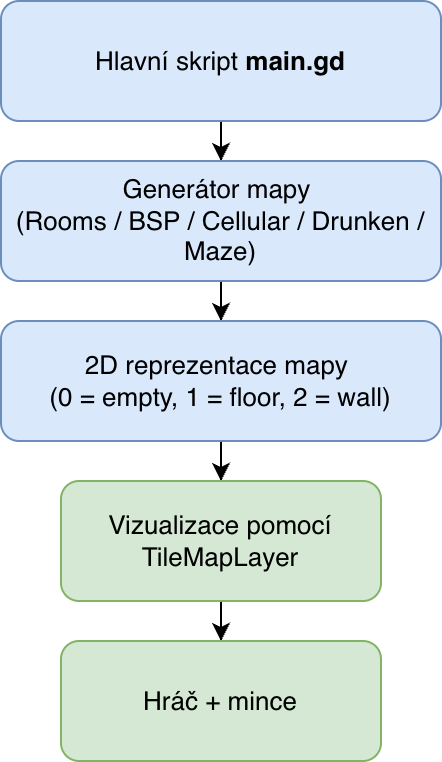
\includegraphics[width=0.4\textwidth]{figures/generator_architecture.png}
\caption{Schéma architektury systému generování dungeonových map}
\label{fig:generator_architecture}
\end{figure}

\subsubsection{Vizualizace mapy a hráče}
Pro vizualizaci generovaných map aplikace využívá grafické prvky, takzvané assety. Tyto assety slouží především k~přehlednému zobrazení struktury generované mapy a~usnadňují orientaci uživatele. Vizualizace zahrnuje grafiku podlahy, stěn, postavy hráče a~sbíratelných objektů.

Mapu zobrazuje komponenta \texttt{TileMapLayer}. Po dokončení generování skript předá datovou reprezentaci mapy funkci \\\texttt{\_draw\_map\_animated()}, která ji postupně převádí na odpovídající dlaždice, řádek po řádku s~krátkou prodlevou mezi jednotlivými řádky. Aplikace mapuje jednotlivé typy buněk na konkrétní grafické prvky představující podlahu nebo stěnu. Tento způsob postupného vykreslování sice není nezbytný z~hlediska samotného generování, ale výsledná vizualizace působí přívětivěji.

Součástí prototypu je také jednoduchá reprezentace hráče, která slouží především k~ověření průchodnosti mapy. Umísťování hráče zajišťuje funkce \\ \texttt{\_place\_player\_on\_floor()}, která nejprve pomocí prohledávání do šířky (BFS) nalezne největší souvislou oblast podlahových dlaždic. V~této oblasti poté hledá pozici s~volným okolím $3 \times 3$ dlaždic, aby hráč nebyl ihned po vytvoření mapy zaseknut ve stěně. Pokud taková pozice neexistuje, funkce jako záložní řešení vybere náhodnou dlaždici z~největší oblasti. S~hráčem se lze jednoduše pohybovat pomocí kláves W, A, S, D. Po mapě se uživatel může pohybovat pravým tlačítkem myši, aniž by ovlivnil pozici hráče, pro návrat k~původní pozici slouží klávesa R.

Pro doplnění testovacího prostředí implementace přidává do mapy sběratelné objekty ve formě mincí. Funkce \texttt{\_place\_coins\_on\_floor()} náhodně rozmístí 5 až 50 mincí na podlahové dlaždice v~největší souvislé oblasti mapy. Pokud hráč posbírá všechny mince, automaticky se vygeneruje nová mapa se stejnými parametry, jako v~případě předchozího generování. Tyto prvky neslouží jako hlavní součást PCG, jedná se pouze o~grafické doplnění.

Implementace využívá volně dostupný balíček 2D Pixel Dungeon Asset Pack, jehož autorem je grafik vystupující pod jménem Pixel\_Poem. Tento balíček obsahuje základní sadu grafických prvků určených právě pro tvorbu dungeonových 2D her \cite{pixel_dungeon_asset}.

Použité assety mají podobu pixelové grafiky v~top-down perspektivě, tedy seshora dolů, a~svým návrhem přímo odpovídají práci s~dlaždicovou mapou, kterou engine využívá. Balíček je volně dostupný a~lze jej využít v~nekomerčních i~komerčních projektech.

Grafická vrstva -- hráč a~mince -- slouží pouze jako podpůrný nástroj pro vizualizaci výsledků generování.

\subsubsection{Ovládání generování a zobrazení statistik}

Uživatelské rozhraní umožňuje výběr konkrétní generovací metody a~nastavení základních parametrů mapy, šířky a~výšky.

Rozhraní obsahuje dvě hlavní tlačítka, \textit{Generate} a~\textit{Benchmark}. Po stisknutí tlačítka \textit{Generate} skript na základě uživatelské volby vybere příslušný generátor pomocí příkazu \texttt{match} a~zavolá jeho funkci \\ \texttt{generate(width, height)}. Dobu generování měří funkce \\ \texttt{Time.get\_ticks\_usec()} výhradně při volání generovací funkce, nikoli při vizualizaci mapy nebo umísťování herních objektů, čímž vykreslování neovlivní naměřený čas. Ihned po dokončení generování skript spočítá počet podlahových dlaždic a~procentuální pokrytí mapy a~zobrazí tyto údaje spolu s~časem generování v~uživatelském rozhraní. Výsledná mapa je poté vizualizována postupným vykreslováním jednotlivých řádků.

Tlačítko \textit{Benchmark} automaticky testuje všechny implementované metody. Funkce \texttt{run\_benchmark()} postupně spustí všech pět algoritmů pro každou z~pěti definovaných velikostí map a~každou konfiguraci opakuje desetkrát. V~tomto režimu se mapa nevizualizuje a~herní objekty se neumisťují.

Funkce \texttt{\_log\_results()} po každém běhu uloží výsledky (algoritmus, rozměry, čas generování, pokrytí, počet podlahových dlaždic) do souboru \texttt{results.csv}; její strukturu podrobněji popisuje podkapitola věnovaná metodice měření.

\begin{figure}[H]
\centering
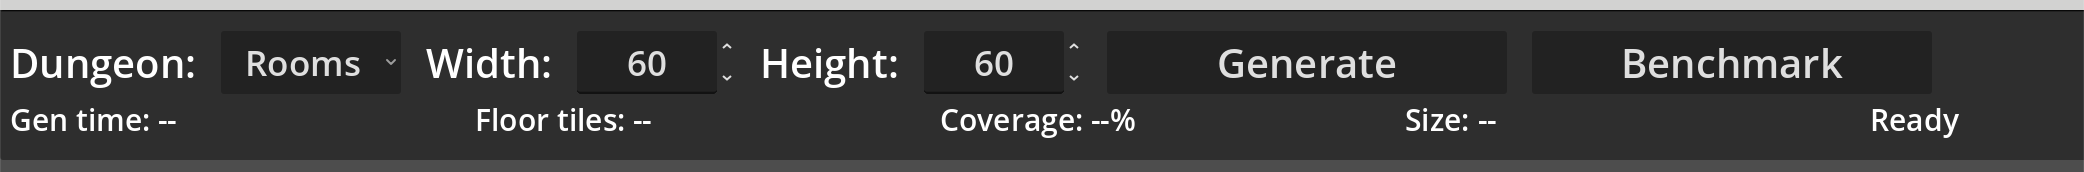
\includegraphics[width=0.8\textwidth]{images/ui.png}
\caption{Uživatelské rozhraní aplikace pro generování map}
\end{figure}


\subsection{Implementace generovacích metod}
Každý algoritmus z~kapitoly~\ref{sec:prehledMetod} je implementován jako samostatný skript v~adresáři \path{res://dungeons/algorithms}.

Všechny generátory sdílejí několik společných implementačních prvků. Každý skript rozšiřuje třídu \texttt{RefCounted}, nemá tedy vazbu na scénu, a~definuje trojici celočíselných konstant pro typy dlaždic: \texttt{TILE\_EMPTY = 0} (prázdný prostor), \texttt{TILE\_FLOOR = 1} (podlaha) a~\texttt{TILE\_WALL = 2} (stěna). Vstupním bodem je vždy statická funkce \texttt{generate(width, height)}, která vrací dvourozměrné pole představující výslednou mapu.

Na začátku funkce \texttt{generate()} každý generátor vytvoří lokální instanci \texttt{RandomNumberGenerator} a~zavolá metodu \texttt{rng.randomize()}, čímž zajistí unikátní průběh náhodných operací bez ovlivnění zbytku aplikace. Následně inicializuje prázdnou mapu o~rozměrech \texttt{width} $\times$ \texttt{height}, kde má každá buňka hodnotu \texttt{TILE\_EMPTY}. Výjimkou je generátor Buněčných automatů, který inicializaci mapy a~náhodnou počáteční výplň provádí v~jednom kroku. Podrobněji tento postup popisuje příslušná podkapitola.

Závěrečným krokem každý generátor doplní stěny funkcí \texttt{\_add\_walls()}, jejíž implementace je ve všech skriptech totožná. Funkce prochází celou mapu a~pro každou dlaždici podlahy kontroluje osm okolních buněk (Mooreovo sousedství). Pokud se v~sousedství nachází buňka \texttt{TILE\_EMPTY}, je změněna na \texttt{TILE\_WALL}. Tímto postupem vznikne souvislé ohraničení všech průchozích částí mapy bez nutnosti generovat stěny explicitně během samotného algoritmu. Kontrola hranic mapy zajišťuje, že se při zápisu stěn nepřistupuje mimo rozsah pole.

\subsubsection{Náhodné umístění místností a~chodeb}

Implementace algoritmu se nachází v~souboru \texttt{rooms\_generator.gd}.

Počet generovaných místností vychází z~celkové plochy mapy podle vzorce \\ \texttt{room\_count = max(5, width * height / AREA\_PER\_ROOM)}. \\ Hodnota konstanty \texttt{AREA\_PER\_ROOM = 360} vychází z~odhadu průměrné plochy, kterou jedna místnost včetně svého okolí v~mapě zabírá. Algoritmus generuje šířku i~výšku místnosti náhodně v~rozmezí 6 až 16 dlaždic, průměrná velikost místnosti tedy činí přibližně $11 \times 11 = 121$ dlaždic. 

Kromě samotné plochy místnosti je však nutné počítat také s~prostorem, který zabírají chodby, stěny a~povinné jednopolíčkové mezery mezi místnostmi. Na základě empirického pozorování je tento faktor přibližně trojnásobkem plochy místnosti, tedy $121 \times 3 \approx 360$ dlaždic na jednu místnost. Na malých mapách tak algoritmus vygeneruje alespoň pět místností, zatímco na velkých mapách počet místností úměrně roste s~plochou. Maximální počet pokusů o~umístění místnosti odpovídá hodnotě \texttt{room\_count * 10}, což zajišťuje dostatečný prostor pro opakované pokusy v~případě kolizí s~již umístěnými místnostmi, a~zároveň zabraňuje nekonečnému cyklování na mapách, kde se požadovaný počet místností nedaří umístit.

Algoritmus reprezentuje každou novou místnost obdélníkem typu \texttt{Rect2} s~náhodně vygenerovanými rozměry a~určí pozici levého horního rohu tak, aby místnost ležela uvnitř hranic mapy a~nezačínala přímo na jejím okraji.

Před přidáním nové místnosti do mapy algoritmus zkontroluje překryv se všemi dříve umístěnými místnostmi. Tato kontrola používá metodu \texttt{grow(1).intersects(other)}, což znamená, že se testuje nejen skutečný průnik obdélníků, ale i~jejich rozšíření o~jednu dlaždici na každou stranu. V~praxi tak mezi dvěma místnostmi vždy zůstává alespoň jednopolíčková mezera. Pokud by se nová místnost překrývala s~některou z~již existujících, algoritmus ji zahodí a~pokračuje dalším pokusem.

V~případě, že nová místnost překryv nevykazuje, algoritmus ji přidá do seznamu místností a~zapíše její vnitřní plochu do mapy jako podlahu. Dvojice vnořených cyklů projde všechny buňky uvnitř obdélníku místnosti a~nastaví jejich hodnotu na \texttt{TILE\_FLOOR}.

Každá nová místnost je následně propojena chodbou s~předchozí místností v~pořadí umístění. První místnost je z~tohoto propojování vyloučena, protože v~okamžiku jejího přidání ještě neexistuje žádná jiná místnost. Pro propojení se využívají středy obou místností získané pomocí metody \texttt{get\_center()}. Vlastní vytvoření chodby zajišťuje pomocná funkce \texttt{\_carve\_corridor()}, \\ která mezi dvěma zadanými body vyznačí chodbu tvaru písmene L. Algoritmus náhodně rozhoduje, zda bude chodba nejprve vedena ve vodorovném a~poté ve svislém směru, nebo opačně. Díky tomu výsledné mapy nepůsobí monotónně.

Chodba se neskládá pouze z~jedné dlaždice, ale má nastavitelnou šířku. Implementace nastavuje výchozí hodnotu parametru \texttt{corridor\_width} na 2. Výsledná chodba je tedy široká 2 dlaždice a~při zápisu dlaždic chodby algoritmus kontroluje, zda se zapisované souřadnice nacházejí uvnitř hranic mapy, a~to pomocí pomocné funkce \texttt{\_in\_bounds()}.

\begin{figure}[H]
\centering
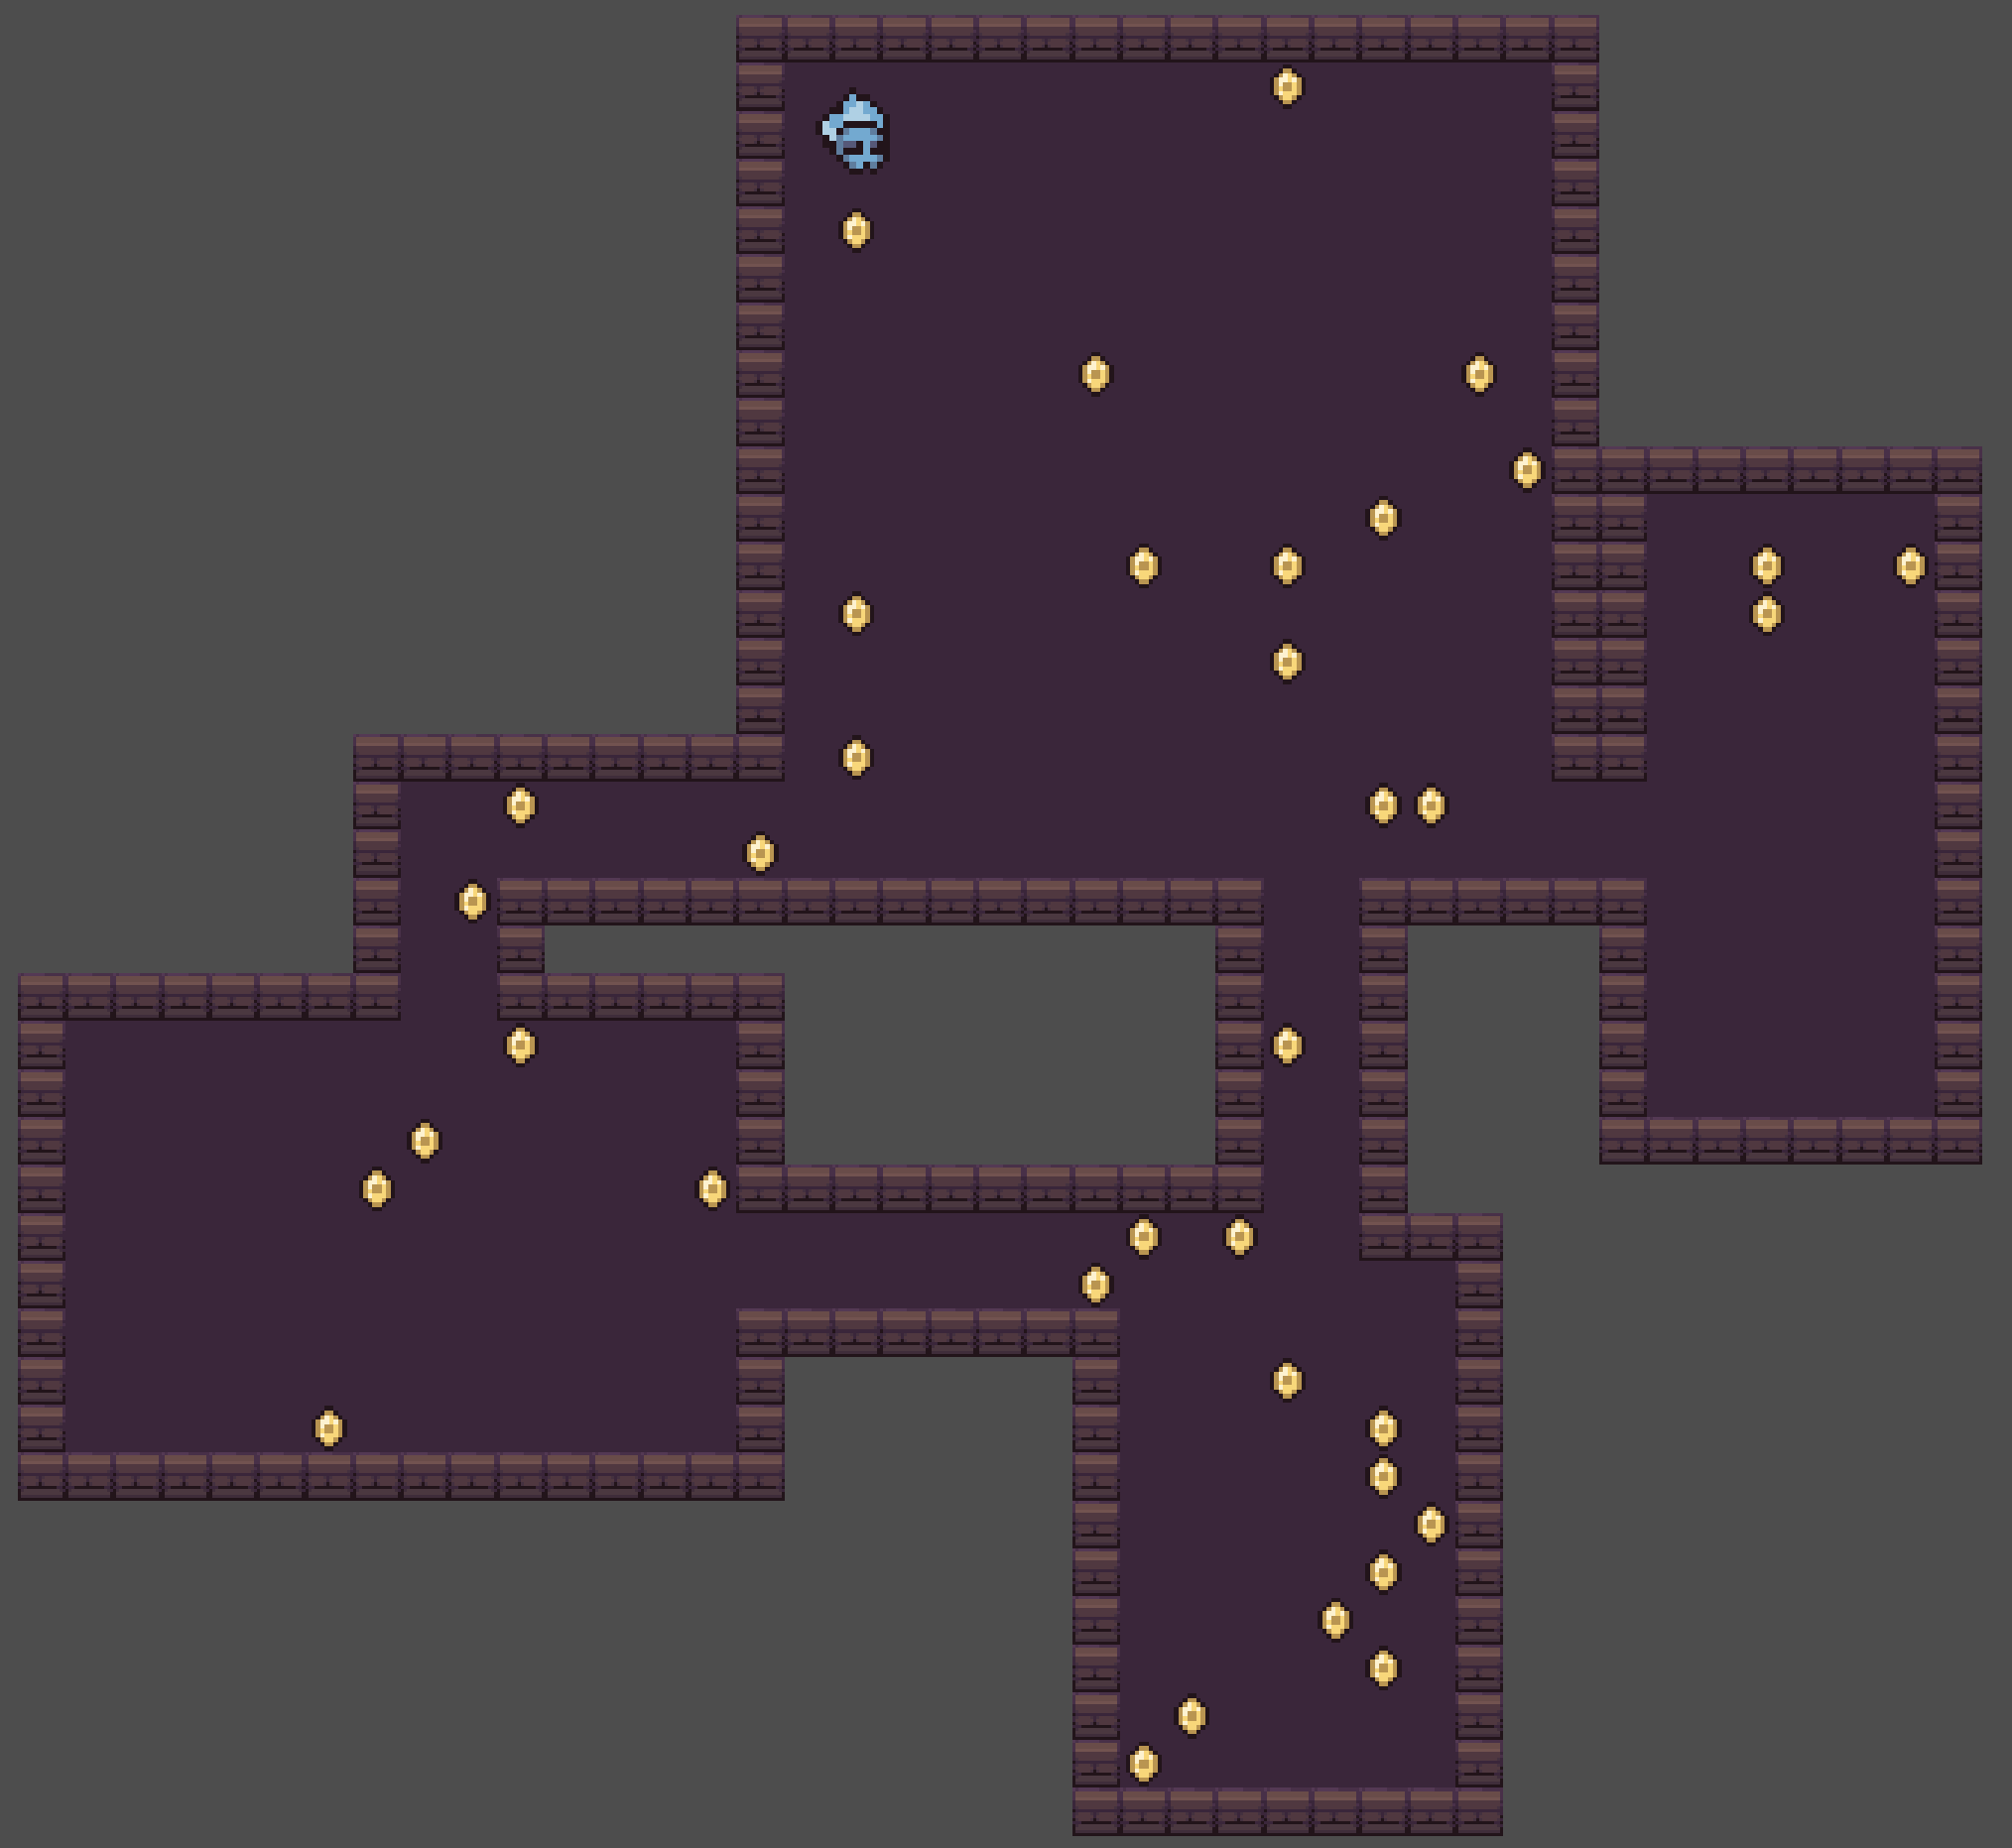
\includegraphics[width=0.7\textwidth]{images/rooms_45x45.png}
\caption{Ukázka mapy generované pomocí algoritmu náhodných místností a~chodeb (45$\times$45)}
\label{fig:rooms_45x45}
\end{figure}

\subsubsection{Binary Space Partitioning}

Implementace metody BSP se nachází v~souboru \texttt{bsp\_generator.gd}.

Pomocná třída \texttt{Branch} reprezentuje stromovou strukturu mapy. \\Každý uzel uchovává svou pozici (\texttt{Vector2i}), velikost (\texttt{Vector2i}) a~náhodné odsazení \texttt{padding} typu \texttt{Vector4i}, jehož složky udávají vzdálenost místnosti od okraje oblasti, náhodně 2 až 3 dlaždice na každé straně. Díky tomuto odsazení nevznikají místnosti těsně u~hranic oblastí a~mezi nimi zůstává dostatečný prostor.

Kořenový uzel pokrývá celou mapu zmenšenou o~jednu dlaždici na každé straně, tedy oblast od pozice $(1, 1)$ o~velikosti $(\texttt{width} - 2) \times (\texttt{height} - 2)$. Tím zůstane na okraji mapy jednopolíčkový rámec.

Rekurzivní dělení prostoru provádí metoda \texttt{split(min\_size, rng)}. \\Algoritmus určuje směr řezu deterministicky. Pokud je výška oblasti větší nebo rovna šířce (\texttt{size.y >= size.x}), dělí se horizontálně, jinak vertikálně. Algoritmus ukončí dělení, pokud by výsledné podoblasti byly menší než \texttt{min\_size $\times$ 2}. Algoritmus volí pozici řezu náhodně v~rozmezí 35--65\,\% délky dělené části, takže vzniklé podoblasti nemusí být stejně velké.

Generátor volá funkci \texttt{split()} s~hodnotou konstanty \texttt{MIN\_SIZE = 13} a~rekurzivně dělí prostor tak dlouho, dokud to velikost oblasti umožňuje. Počet výsledných listových uzlů tedy není fixní, ale závisí na rozměrech mapy. Na větších mapách vzniká více oblastí a~tím i~více místností.
V~každém listu algoritmus vykreslí místnost odpovídající ploše uzlu zmenšené o~jeho odsazení \texttt{padding}.

Teprve po dokončení celého stromu metoda \\\texttt{get\_corridor\_pairs()} vrátí chodby. Prochází strom rekurzivně a~pro každý vnitřní uzel vybere první listový uzel z~levého a~pravého podstromu a~uloží dvojici jejich středů. Metoda \texttt{get\_room\_center()} vypočítá středy místností se zohledněním odsazení \texttt{padding}, takže výsledný bod leží vždy uvnitř skutečné průchozí plochy místnosti, nikoliv jen v~geometrickém středu celé podoblasti. Každá chodba má tvar písmene L, nejprve vede ve vodorovném, a~poté ve svislém směru. Chodba je široká 2 dlaždice.

\begin{figure}[H]
\centering
\includegraphics[width=0.7\textwidth]{images/bsp_45x45.png}
\caption{Ukázka mapy generované pomocí algoritmu BSP (45$\times$45)}
\label{fig:bsp_45x45}
\end{figure}

\subsubsection{Metoda Náhodné procházky}

Metoda Náhodné procházky se nachází v~souboru \\ \texttt{drunkards\_generator.gd}. Algoritmus začíná ve středu mapy na pozici \\ \texttt{width/2}, \texttt{height/2}. Algoritmus ihned vytvoří kolem počáteční pozice oblast podlahy o~velikosti $3 \times 3$ dlaždic pomocí funkce \texttt{\_carve\_3x3()}. Cílový počet podlahových dlaždic činí 50\,\% celkové plochy mapy podle vzorce~(\ref{eq:drunkards_target}), kde konstanta \textit{TARGET\_COVERAGE} má hodnotu 50.

\begin{equation}
\label{eq:drunkards_target}
\textit{cílový\_počet} = \frac{\textit{width} \times \textit{height} \times \textit{TARGET\_COVERAGE}}{100}
\end{equation}

Algoritmus běží v~cyklu, který pokračuje, dokud počet podlahových dlaždic nedosáhne cílového počtu. V~každém kroku algoritmus náhodně zvolí jeden ze čtyř směrů (nahoru, dolů, doleva, doprava) a~posune pozici generátoru o~jednu dlaždici. Funkce \texttt{clamp()} ji omezuje tak, aby zůstávala alespoň 2 dlaždice od okraje mapy. Tato rezerva zajistí, že i~při vykreslování oblastí $3 \times 3$ nepřekročí hranice pole.

Algoritmus rozlišuje dva typy vykreslování. Každých 15 až 25 kroků (náhodně volený interval) algoritmus vytvoří na aktuální pozici oblast $3 \times 3$ dlaždic, která představuje malou místnost. V~ostatních krocích vykreslí pouze oblast $2 \times 2$ dlaždic, což odpovídá chodbovému úseku. Obě varianty zajišťuje jediná pomocná funkce \texttt{\_carve\_area()}, které se předá požadovaná velikost oblasti (3 nebo 2). Funkce zapisuje podlahu pouze tam, kde dosud podlaha nebyla, a~vrací počet nově vytvořených dlaždic, aby mohl být průběžně aktualizován celkový počet.

Průchodnost celé mapy je zaručena tím, že veškerý průchozí prostor vzniká z~jedné souvislé procházky. Díky pevně stanovenému cílovému podílu podlahy je pokrytí mapy pro danou velikost relativně stabilní. Variabilita se projevuje především ve tvaru a~rozmístění vytvořených prostorů.

\begin{figure}[H]
\centering
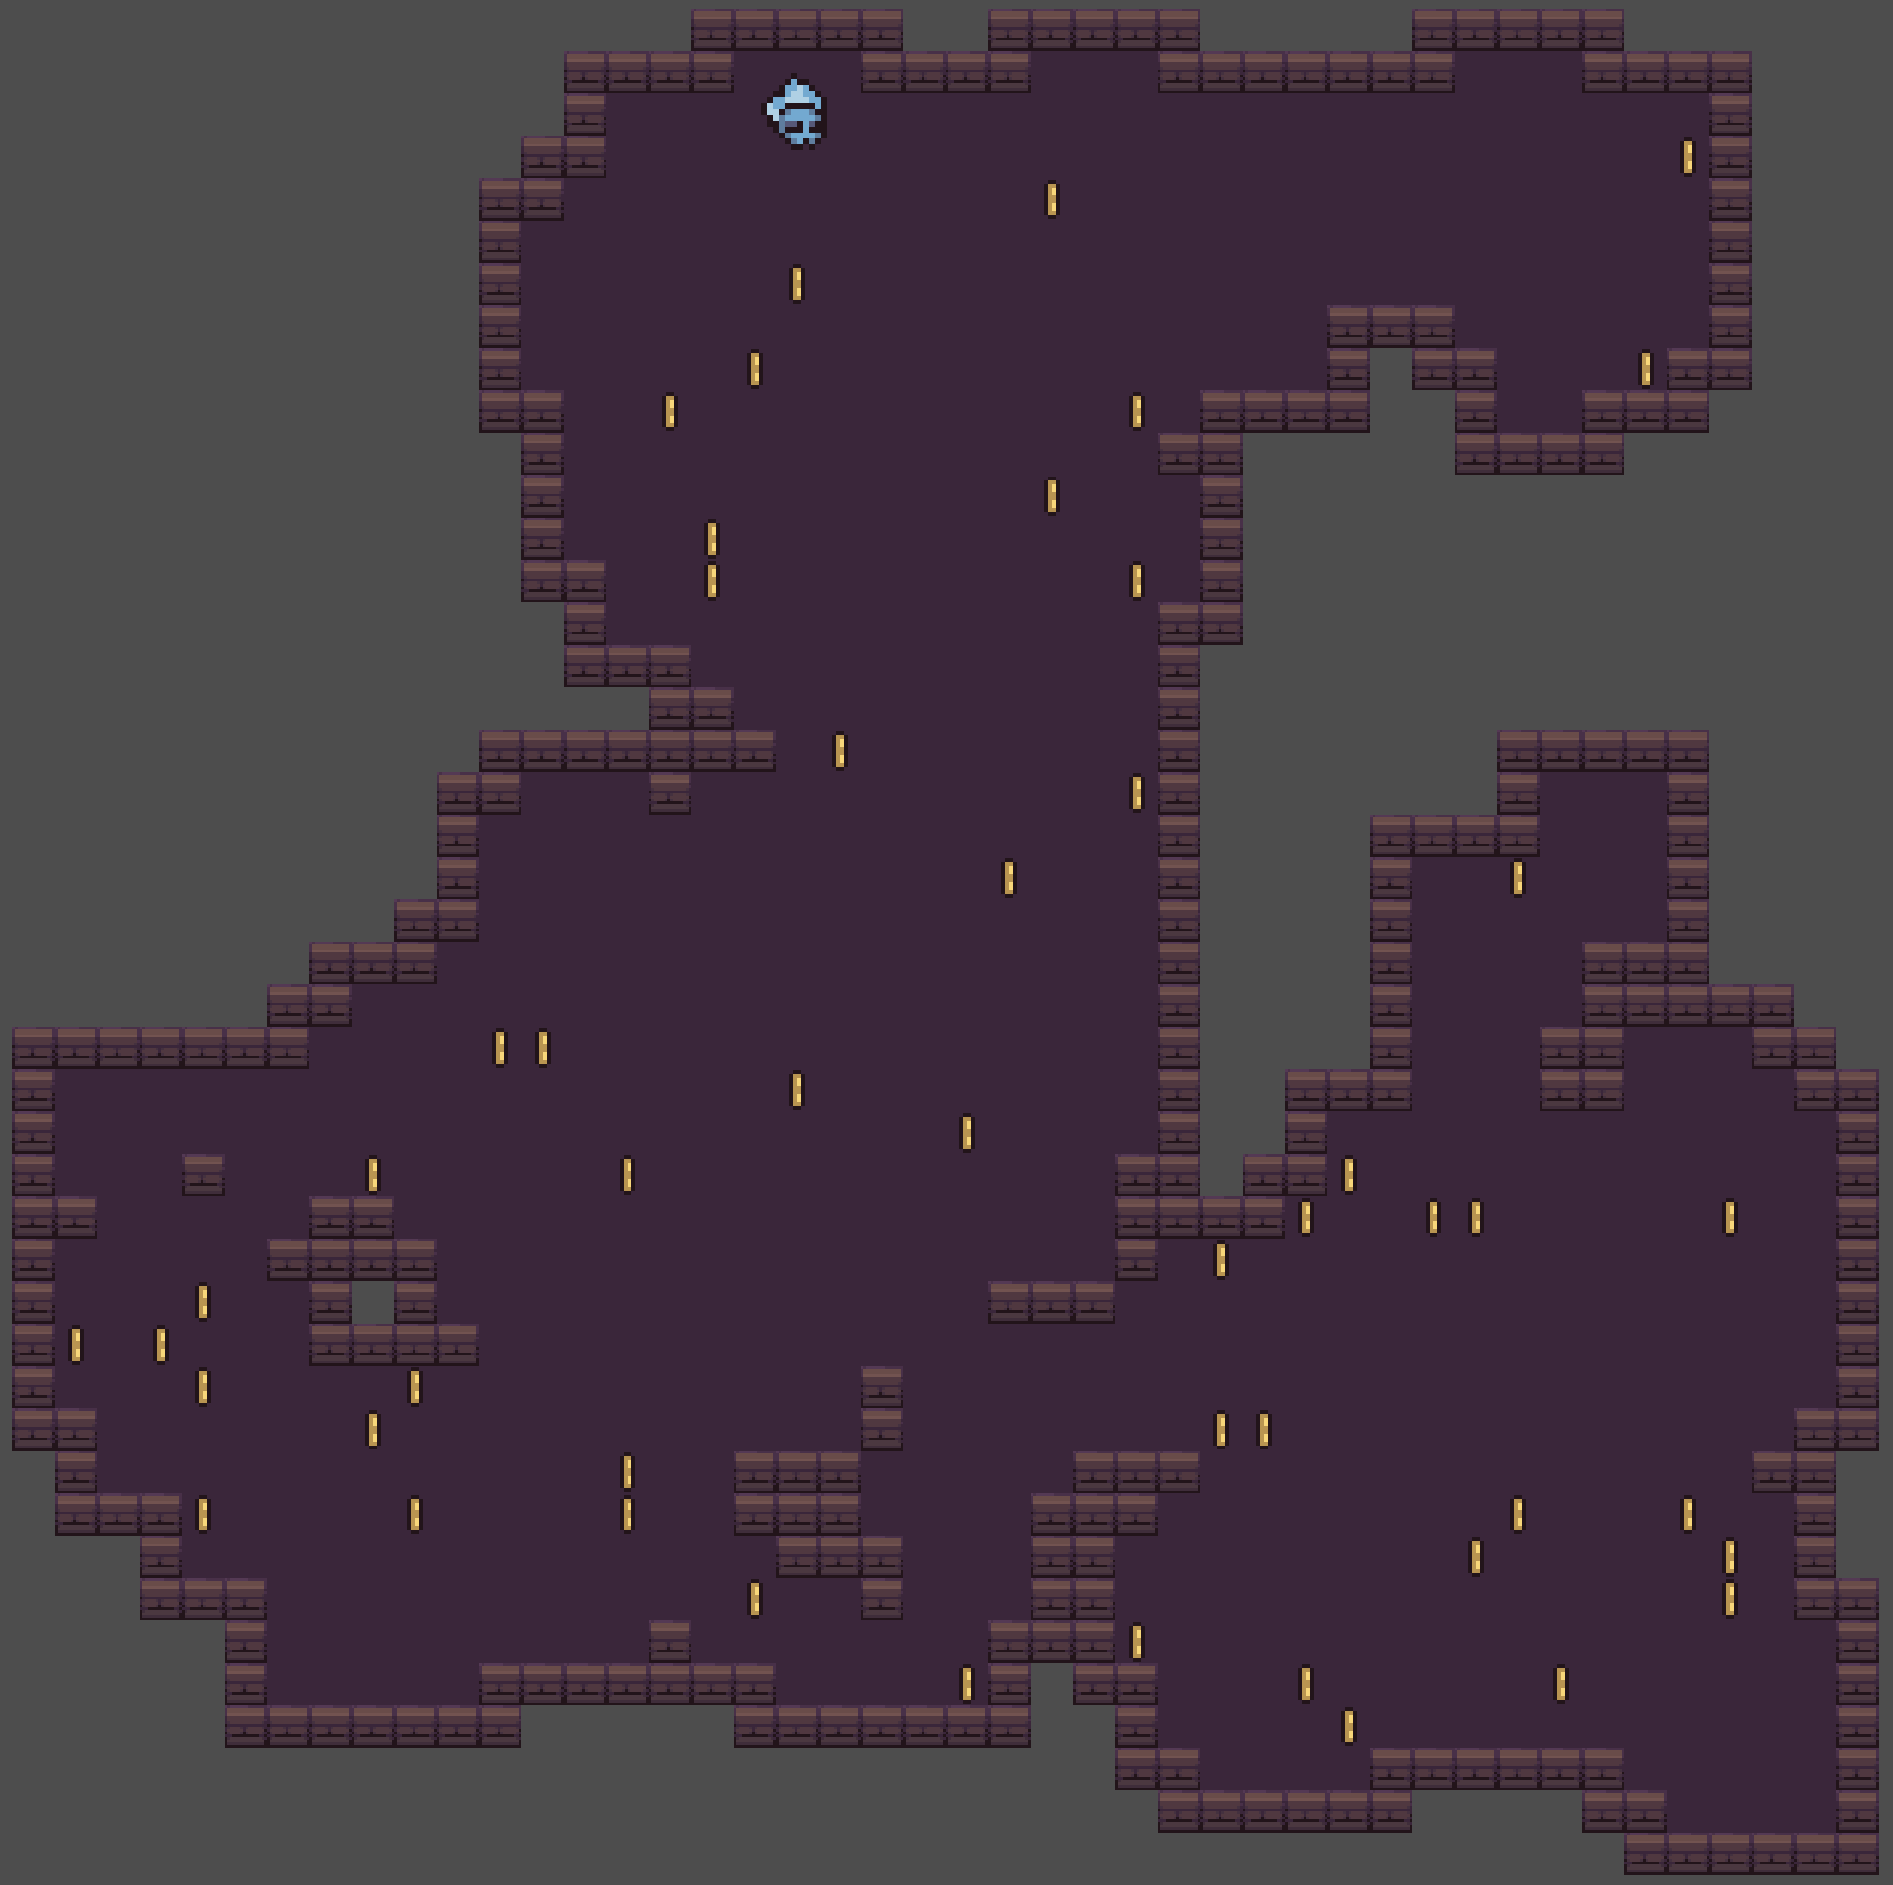
\includegraphics[width=0.7\textwidth]{images/drunkards_45x45.png}
\caption{Ukázka mapy generované pomocí algoritmu Náhodné procházky (45$\times$45)}
\label{fig:drunkards_45x45}
\end{figure}

\subsubsection{Buněčné automaty}

Implementace Buněčných automatů je v~souboru \texttt{cellular\_generator.gd}. 

V~první fázi algoritmus náhodně nastaví každou vnitřní buňku mapy na podlahu s~pravděpodobností \texttt{FILL\_PROBABILITY = 0.45}, tedy 45\,\%. Buňky na okraji mapy (první a~poslední řádek a~sloupec) zůstávají vždy prázdné, čímž vznikne pevný rámec, který zabraňuje rozšíření jeskynních prostor až k~hranicím pole.

Algoritmus provede celkem 5 simulačních kroků (konstanta \texttt{SIMULATION\_STEPS}). V~každém kroku algoritmus vytvoří novou mapu, aby se průběžné změny nepromítaly do výpočtu sousedů v~témže kroku. Pro každou buňku funkce \texttt{\_count\_floor\_neighbours()} spočítá počet podlahových sousedů v~Mooreově okolí (osm přilehlých buněk). Pokud je tento počet alespoň 4, buňka se stane podlahou, v~opačném případě zůstane prázdná. Okrajové buňky ve všech krocích zůstávají prázdné.

Opakováním tohoto pravidla se náhodný šum postupně vyhladí do organických tvarů připomínajících jeskynní systémy. Volba počáteční pravděpodobnosti 45\,\% a~prahu 4 sousedů představuje kompromis mezi dostatečně otevřenými prostory a~přirozeně působícími stěnami. Při vyšší hodnotě by vznikaly příliš velké otevřené části, při nižší by byly oblasti méně průchozí, protože by velká část buněk tvořila stěny.

U map generovaných touto metodou se mohou vyskytovat izolované průchozí oblasti, protože algoritmus nezaručuje souvislost prostoru. Z~tohoto důvodu bylo při umisťování hráče nutné zohlednit průchozí plochu a~upřednostnit umístění do největší spojité oblasti mapy, což implementace nakonec zahrnula do všech metod.

\begin{figure}[H]
\centering
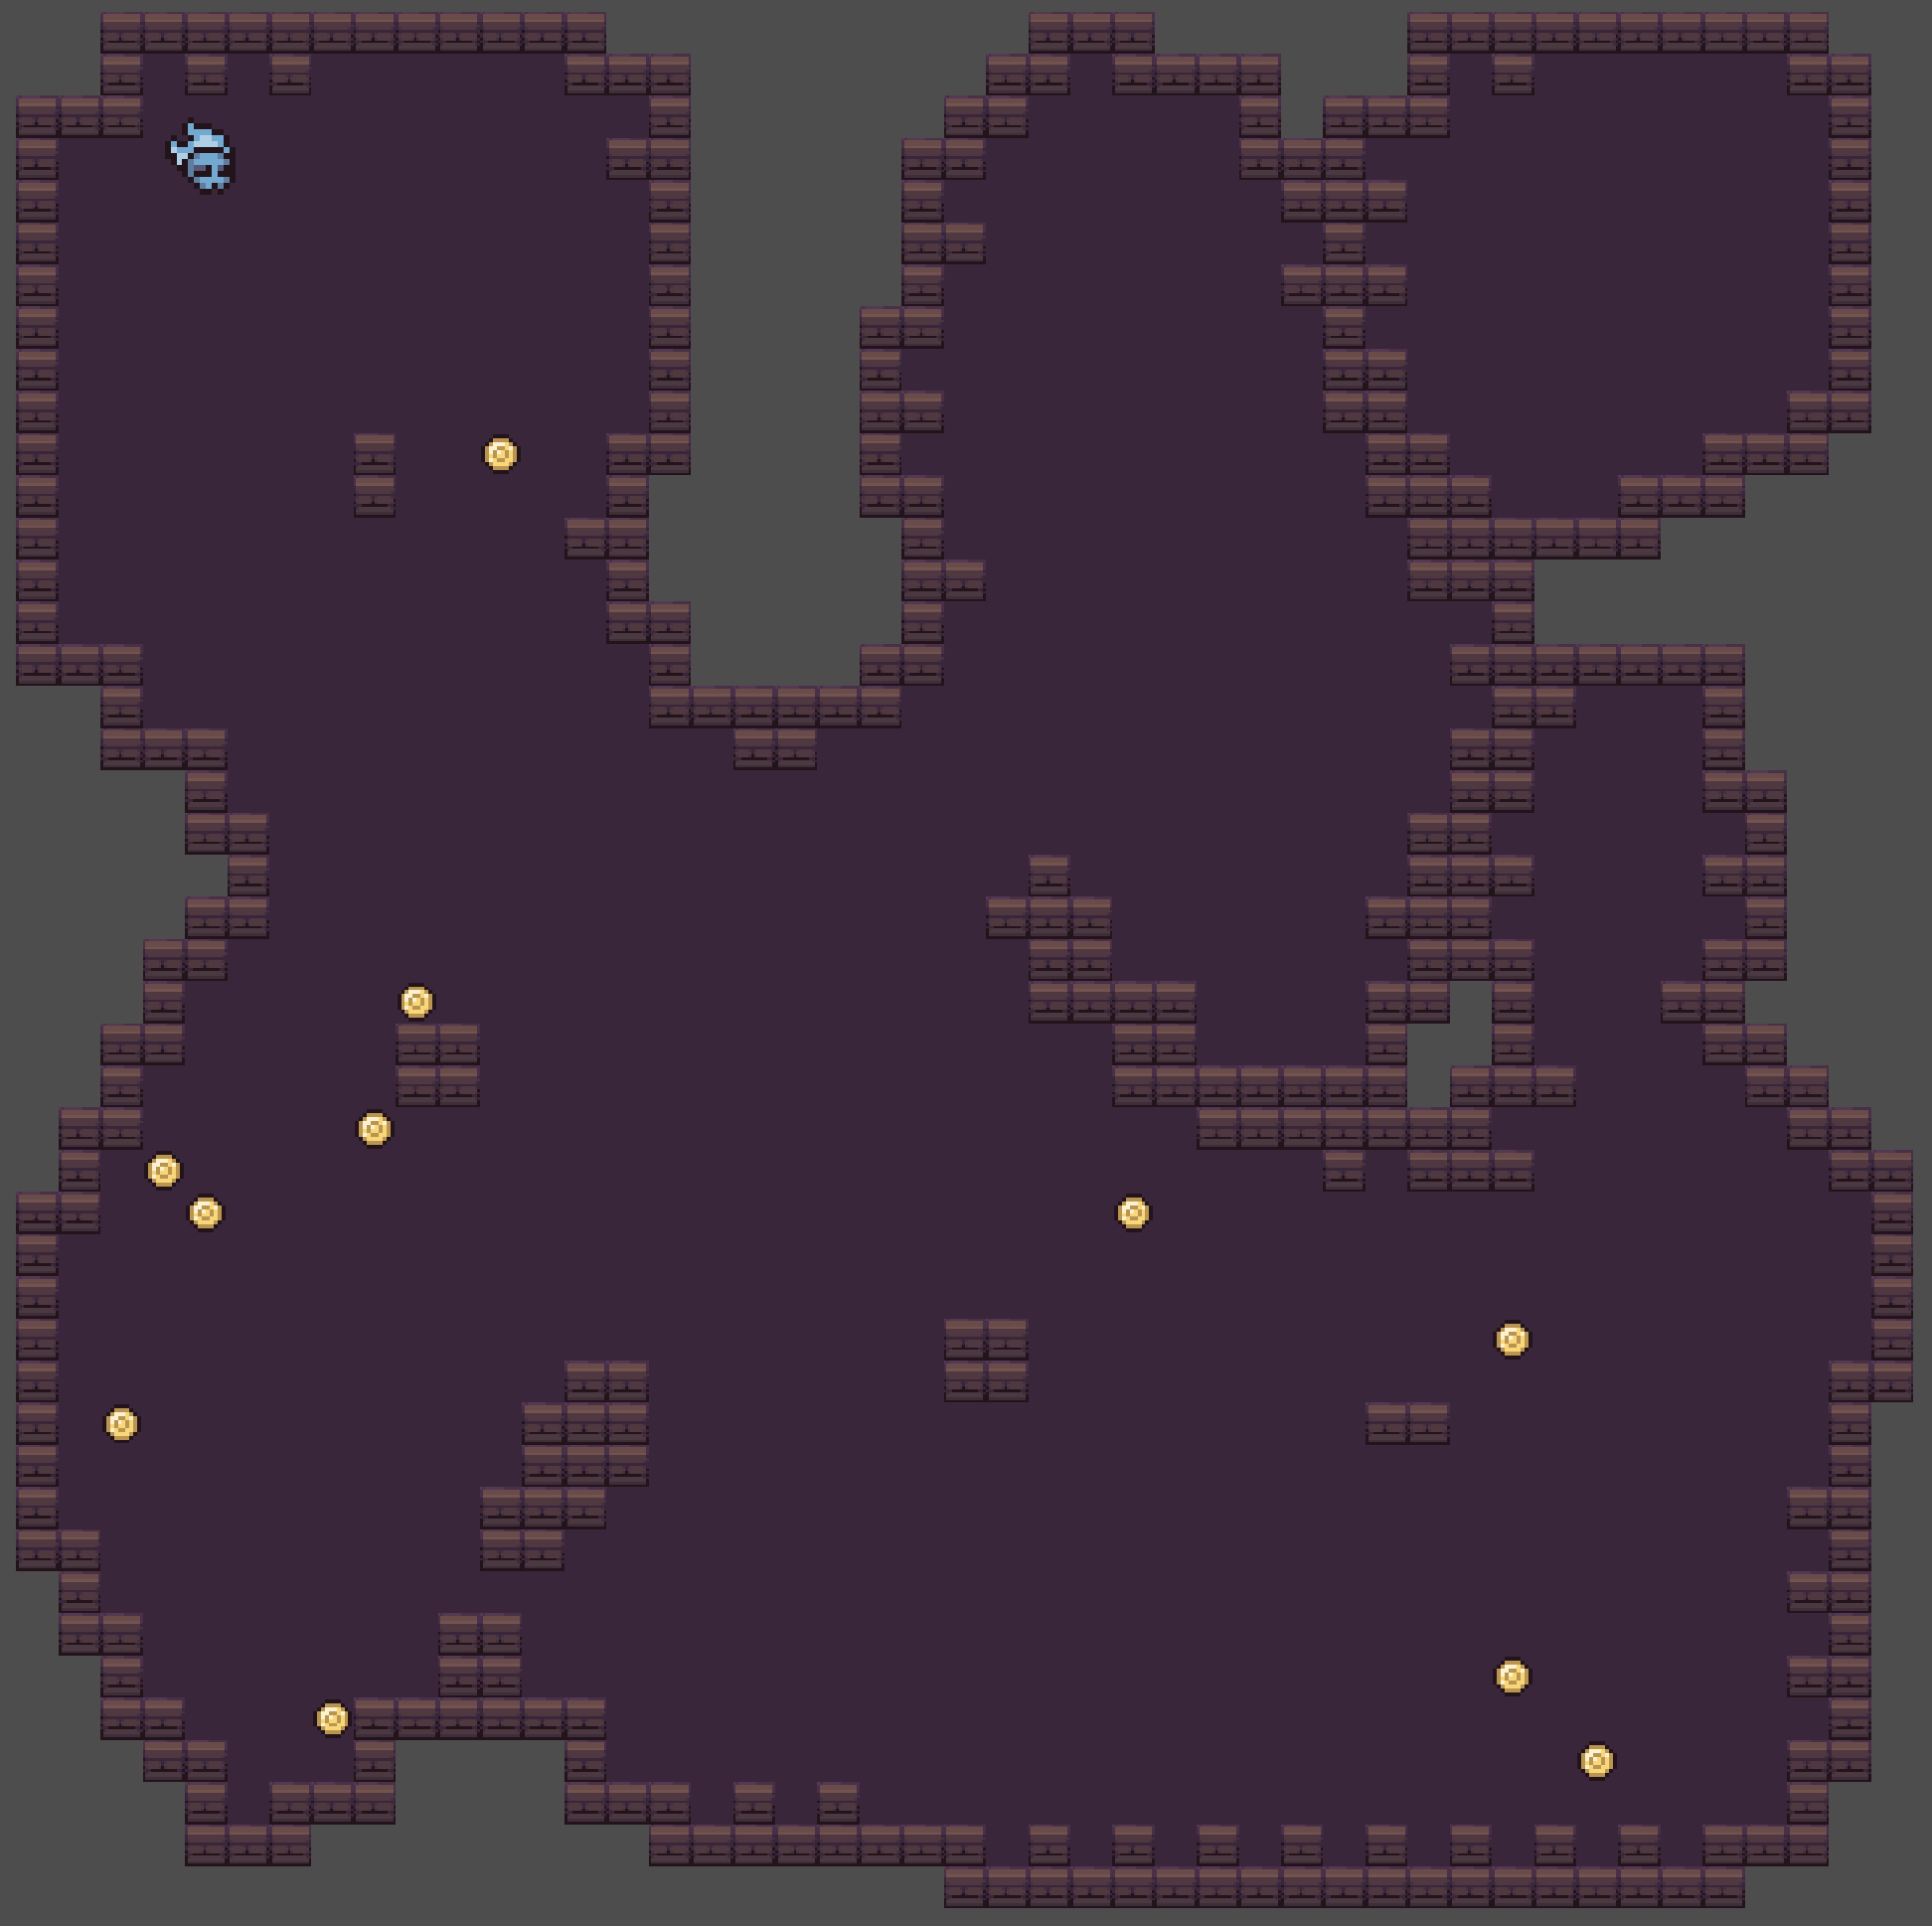
\includegraphics[width=0.7\textwidth]{images/cellular_45x45.png}
\caption{Ukázka mapy generované pomocí algoritmu Buněčných automatů (45$\times$45)}
\label{fig:cellular_45x45}
\end{figure}

\subsubsection{Metoda Bludiště}

Implementace Bludiště se nachází v~souboru \texttt{maze\_generator.gd}.

Implementace metody vychází z~algoritmu \textit{recursive backtracker} (prohledávání do hloubky se zásobníkem). Algoritmus nejprve rozdělí mapu na mřížku abstraktních buněk. Každá buňka zabírá $2 \times 2$ dlaždic podlahy a~mezi sousedními buňkami je jednodlaždicová mezera, takže na jednu buňku připadá úsek $3 \times 3$ dlaždic. Počet buněk závisí na rozměrech mapy, kde odečtení 2 zohledňuje jednodlaždicový okraj mapy na obou stranách:
\begin{equation}
    \texttt{cells\_w} = \max\!\Bigl(1,\, \Bigl\lfloor\frac{\texttt{width} - 2}{3}\Bigr\rfloor\Bigr), \qquad
    \texttt{cells\_h} = \max\!\Bigl(1,\, \Bigl\lfloor\frac{\texttt{height} - 2}{3}\Bigr\rfloor\Bigr).
\end{equation}

Stav každé buňky představuje bitová maska čtyř stěn (\texttt{N = 1}, \texttt{E = 2}, \texttt{S = 4}, \texttt{W = 8}), na začátku jsou všechny stěny přítomné. Algoritmus startuje v~buňce $(0, 0)$ a~v~každém kroku náhodně vybere nenavštíveného souseda. 
Ze společné stěny algoritmus odstraní příslušný bit na obou stranách, například při pohybu na sever se z~aktuální buňky odstraní bit \texttt{N} a~ze sousední buňky se odstraní bit \texttt{S}. Pokud aktuální buňka nemá žádného nenavštíveného souseda, algoritmus se vrací zpět po zásobníku. Průchod končí, jakmile algoritmus navštíví všechny buňky.

Výsledkem je takzvané perfektní bludiště, ve kterém mezi libovolnými dvěma buňkami existuje právě jedna cesta. Po dokončení prohledávání algoritmus převede buněčnou reprezentaci na dlaždicovou mapu. Každou buňku vykreslí jako oblast $2 \times 2$ podlahových dlaždic na pozici $(1 + \texttt{cx} \cdot 3,\; 1 + \texttt{cy} \cdot 3)$. Tam, kde algoritmus stěnu odstranil, jednodlaždicovou mezeru mezi sousedními buňkami rovněž vyplní podlahou o~šířce 2 dlaždic, čímž vznikne průchozí koridor.

\begin{figure}[H]
\centering
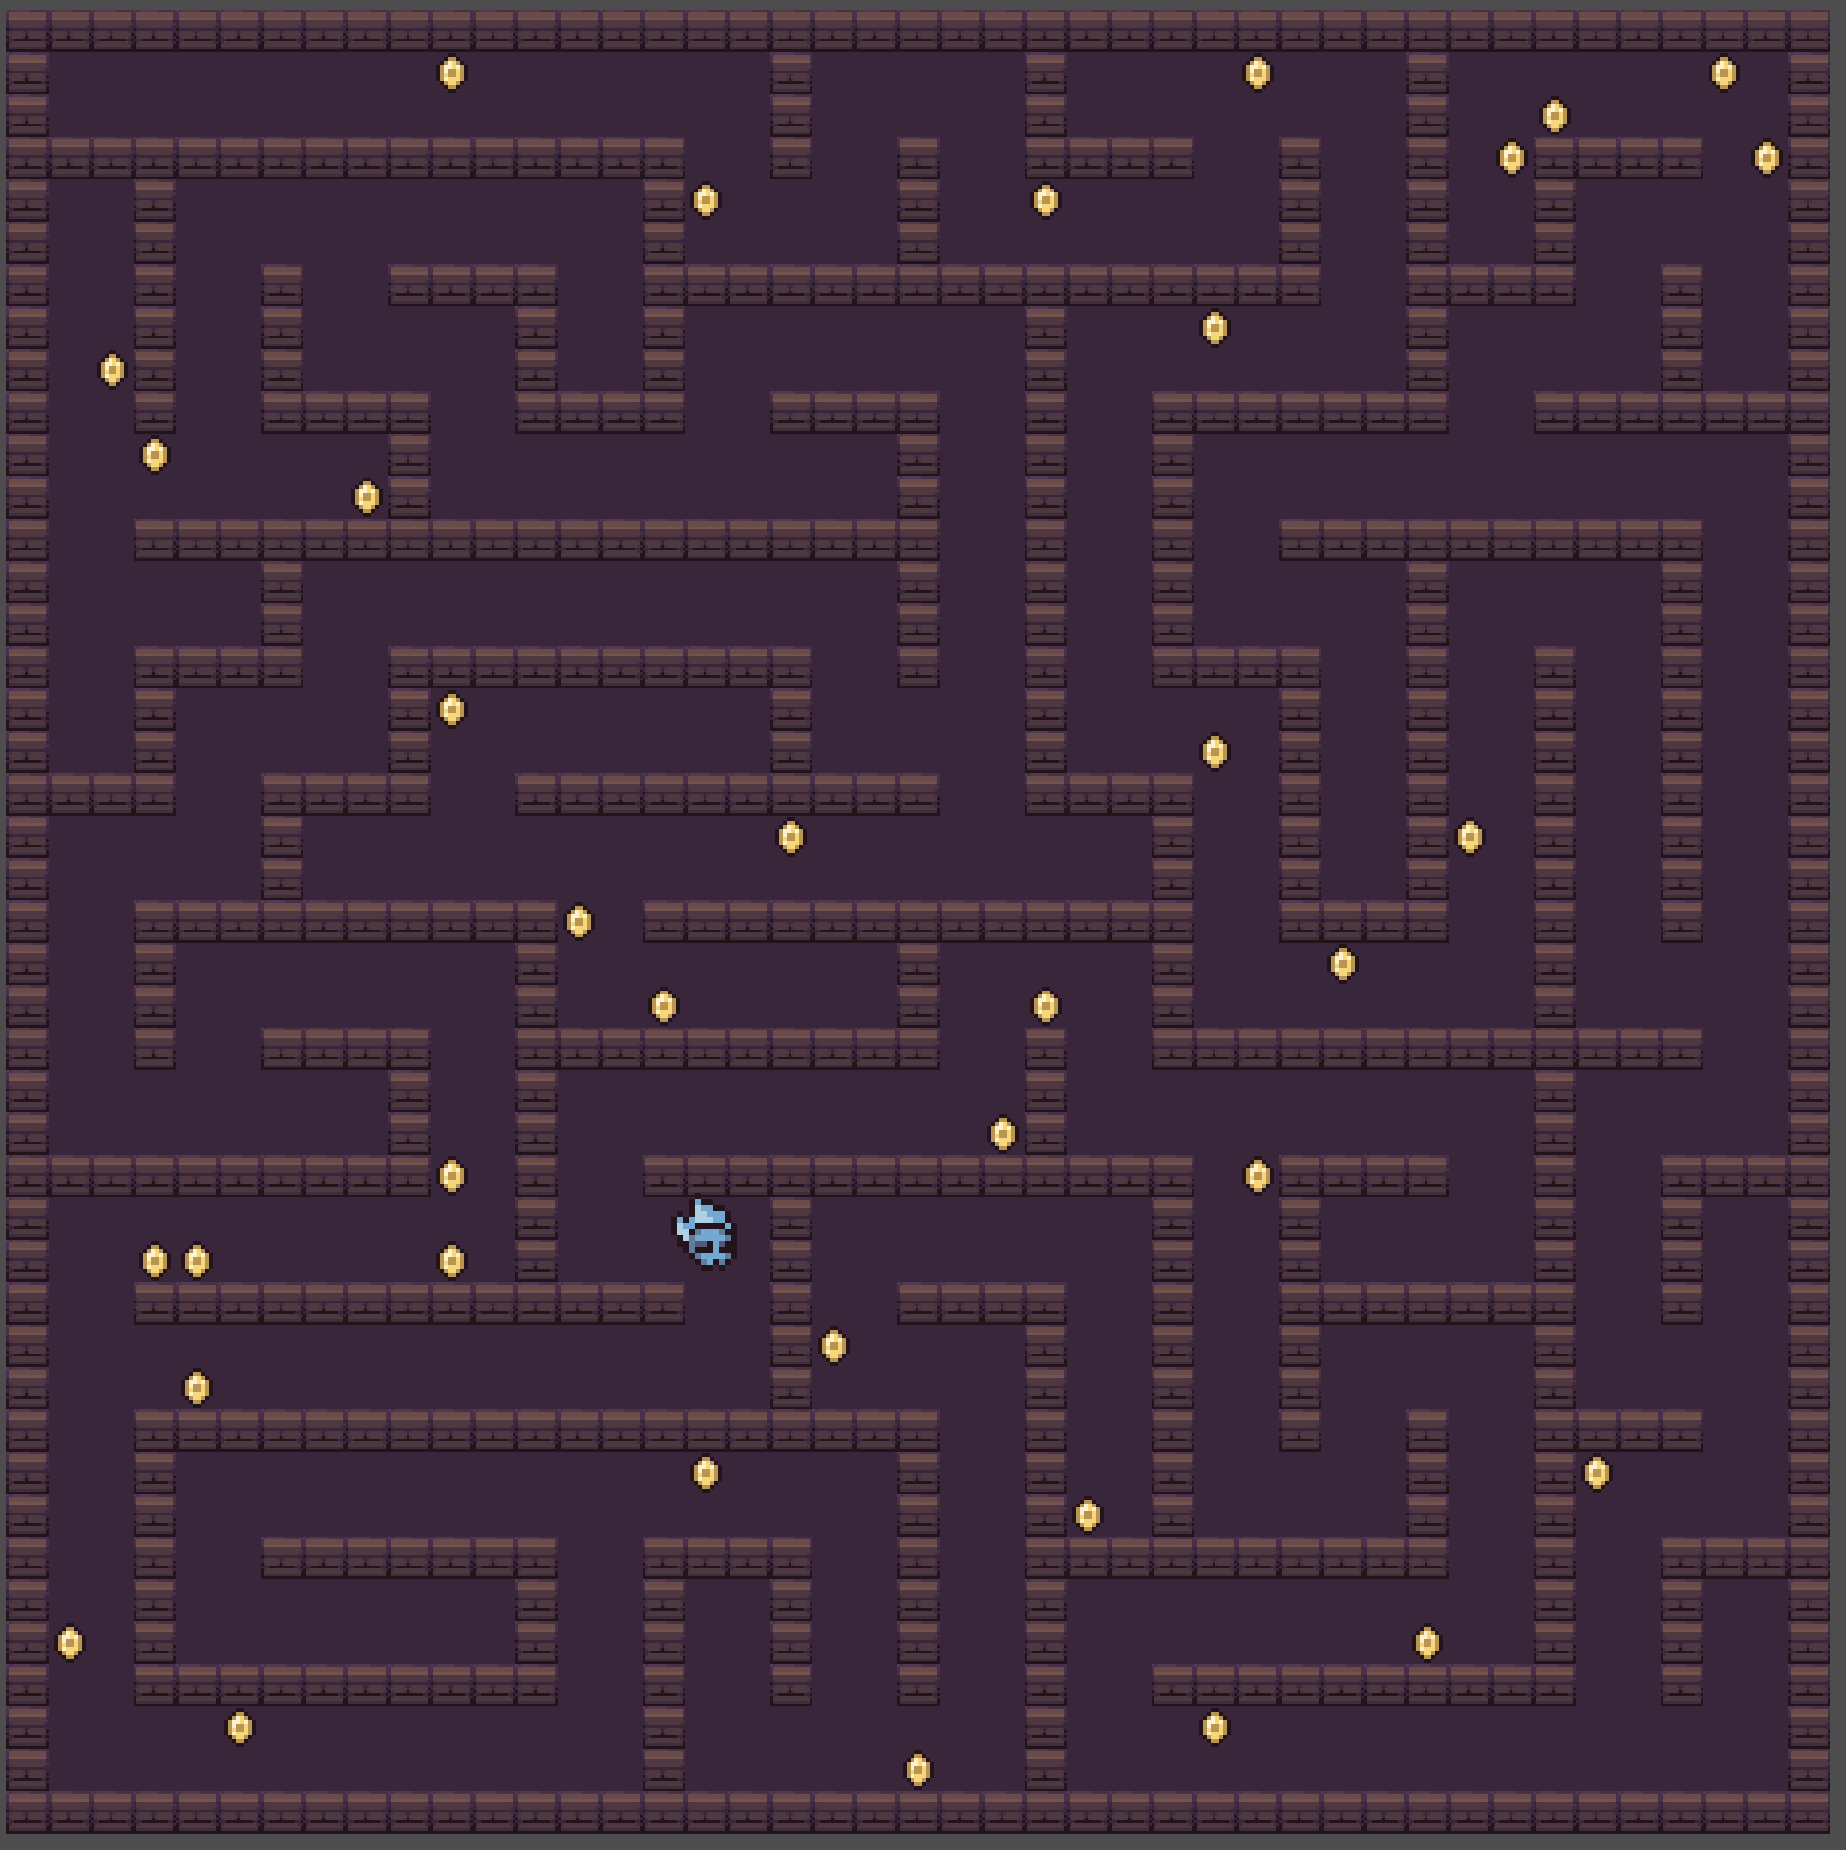
\includegraphics[width=0.7\textwidth]{images/maze_45x45.png}
\caption{Ukázka mapy generované pomocí algoritmu Bludiště (45$\times$45)}
\label{fig:maze_45x45}
\end{figure}


\subsection{Metodika měření a vyhodnocení}

Benchmarkový režim spouští všechny algoritmy pro pět velikostí map: 20$\times$50, 60$\times$60, 70$\times$30, 100$\times$100 a~150$\times$150 dlaždic. Tyto velikosti pokrývají jak malé, tak velké rozměry a~umožňují posoudit vliv tvaru mapy (čtverec versus obdélník) na chování algoritmů. Pro každou kombinaci algoritmu a~velikosti mapy generování proběhne opakovaně v~deseti nezávislých bězích. Benchmark proběhl celkem 5$\times$, čímž vzniklo celkem 1250 záznamů.

Funkce \texttt{Time.get\_ticks\_usec()} zajišťuje měření času s~mikrosekundovou přesností. Měří se výhradně čas funkce \texttt{generate(width, height)} příslušného algoritmu. Vizualizace mapy, vykreslování dlaždic, umisťování hráče a~další operace nejsou součástí měřeného intervalu. Výsledný čas se převede na milisekundy.

Každý běh zahrnuje následující metriky:
\begin{itemize}
\item \textbf{čas generování} (\texttt{gen\_time\_ms}) -- doba trvání samotného algoritmu \\ v~milisekundách
\item \textbf{počet podlahových dlaždic} (\texttt{floor\_tiles}) -- celkový počet podlahových dlaždic ve výsledné mapě
\item \textbf{pokrytí} (\texttt{coverage}) -- podíl podlahových dlaždic z~celkového počtu buněk mapy, vyjádřený v~procentech:
\begin{equation}
    \texttt{coverage} = \frac{\text{floor\_tiles}}{\text{width} \times \text{height}} \times 100
\end{equation}
\end{itemize}

Aplikace průběžně ukládá naměřené hodnoty každého běhu do souboru \texttt{results.csv}. 
Každý záznam obsahuje název algoritmu, rozměry mapy, pořadí běhu, čas generování, pokrytí a~počet podlahových dlaždic.

Naměřená data vyhodnocuje samostatný skript \\ \texttt{result\_analyser.py} v~jazyce Python s~využitím knihoven \texttt{pandas} \\ a~\texttt{matplotlib}. 
Skript načte soubor \texttt{results.csv} a~pro každou kombinaci algoritmu a~velikosti mapy vypočítá souhrnné statistiky -- průměr, směrodatnou odchylku, minimum a~maximum času generování i~pokrytí. Skript tyto statistiky uloží do souboru \texttt{results\_summary.csv}. Následně skript automaticky vygeneruje sadu grafů: sloupcové grafy průměrného času a~pokrytí pro jednotlivé algoritmy, škálovací křivky v~závislosti na velikosti mapy, boxploty rozložení hodnot a~bodový graf kompromisu mezi rychlostí a~pokrytím. Všechny grafické výstupy použité v~následující kapitole tento skript vygeneroval.

\section{Výsledky}

Všechny grafy v~této kapitole vznikly z~dat naměřených benchmarkovým režimem popsaným v~předchozí podkapitole. Osy a~legendy grafů jsou uvedené v~anglickém jazyce. Názvy algoritmů v~grafech odpovídají anglickým označením \textit{Rooms} (Místnosti), \textit{BSP}, \textit{Drunkard's} (Náhodná procházka), \textit{Cellular} (Buněčné automaty) a~\textit{Maze} (Bludiště). Každý popisek obrázku uvádí český překlad nadpisu grafu.


\subsection{Výsledky jednotlivých algoritmů}

\subsubsection{Místnosti a chodby}

Algoritmus náhodných místností a~chodeb vykazuje nízké časy generování na menších mapách. Na mapě 20$\times$50 dosahuje průměrný čas přibližně 0,88 ms. S~rostoucí velikostí mapy čas narůstá výrazněji. Na mapě 150$\times$150 dosahuje průměrný čas přibližně 26,3 ms.

Pokrytí mapy průchozím prostorem roste s~velikostí mapy. Na menších mapách (20$\times$50, 70$\times$30) se pohybuje v~rozmezí 31--41 \%, na mapě 100$\times$100 činí přibližně 44 \% a~na mapě 150$\times$150 dosahuje přibližně 53 \%.

Variabilita mezi jednotlivými běhy je u~tohoto algoritmu patrná jak v~čase generování, tak v~pokrytí. Pokrytí se mění podle velikosti a~rozmístění náhodně vygenerovaných místností. Na menších mapách, kde vzniká minimálně pět místností, je variabilita pokrytí vyšší.

\begin{figure}[H]
\centering

\includegraphics[width=0.75\textwidth]{images/graphs/rooms_time_by_size.png}
\caption{Místnosti a chodby -- průměrný čas generování podle velikosti mapy}
\label{fig:rooms_time}
\end{figure}

\begin{figure}[H]
\centering

\includegraphics[width=0.75\textwidth]{images/graphs/rooms_coverage_by_size.png}
\caption{Místnosti a chodby -- průměrné pokrytí podle velikosti mapy}
\label{fig:rooms_coverage}
\end{figure}


\subsubsection{Binary Space Partitioning}

Algoritmus BSP vytváří mapy s~dobře definovanými místnostmi a~systematickým propojením. Čas generování roste s~velikostí map, od přibližně 0,81 ms na mapě 20$\times$50 po 20,3 ms na mapě 150$\times$150.

Pokrytí mapy u~BSP roste s~velikostí mapy. Na nejmenší mapě 20$\times$50 činí pokrytí přibližně 46,3 \%, na mapě 150$\times$150 dosahuje hodnot kolem 53,0 \%.

Variabilita času mezi běhy je u~BSP nízká, směrodatné odchylky jsou malé, což odpovídá determinističtější povaze rekurzivního dělení prostoru. Variabilita pokrytí je střední, výrazně totiž závisí na náhodném průběhu dělení, který ovlivňuje počet a~velikost vzniklých místností.

\begin{figure}[H]
\centering

\includegraphics[width=0.75\textwidth]{images/graphs/bsp_time_by_size.png}
\caption{BSP -- průměrný čas generování podle velikosti mapy}
\label{fig:bsp_time}
\end{figure}

\begin{figure}[H]
\centering

\includegraphics[width=0.75\textwidth]{images/graphs/bsp_coverage_by_size.png}
\caption{BSP -- průměrné pokrytí podle velikosti mapy}
\label{fig:bsp_coverage}
\end{figure}


\subsubsection{Náhodná procházka}

Algoritmus Náhodné procházky se od ostatních metod odlišuje především konstantním pokrytím mapy. Výsledné pokrytí se ve všech testovaných konfiguracích pohybuje v~rozmezí 50,0--50,1 \%, což přímo odpovídá implementaci, ve které je cílový počet podlahových dlaždic stanoven pevně. Variabilita pokrytí je tedy prakticky nulová.

Čas generování vykazuje výraznější variabilitu mezi jednotlivými běhy. Na mapě 20$\times$50 se průměrný čas pohybuje kolem 3,3 ms. Na největší mapě 150$\times$150 dosahuje přibližně 74,1 ms. Hodnota 50 \% je přitom nastavitelný parametr a~změnou této konstanty lze dosáhnout libovolného cílového pokrytí.

Náhodná procházka tak představuje algoritmus s~předvídatelným pokrytím, avšak výrazně proměnlivým časem generování. Délka výpočtu závisí na tom, jak efektivně procházka pokrývá nové oblasti.

\begin{figure}[H]
\centering

\includegraphics[width=0.75\textwidth]{images/graphs/drunkards_time_by_size.png}
\caption{Náhodná procházka -- průměrný čas generování podle velikosti mapy}
\label{fig:drunkards_time}
\end{figure}

\begin{figure}[H]
\centering

\includegraphics[width=0.75\textwidth]{images/graphs/drunkards_coverage_by_size.png}
\caption{Náhodná procházka -- průměrné pokrytí podle velikosti mapy}
\label{fig:drunkards_coverage}
\end{figure}


\subsubsection{Buněčné automaty}

Buněčné automaty jsou z~testovaných algoritmů nejpomalejší. Na nejmenší mapě 20$\times$50 trvá generování přibližně 7,1 ms, na mapě 100$\times$100 již 78,3 ms a~na největší mapě 150$\times$150 dosahuje průměrný čas přibližně 178,8 ms. Hlavní příčinou je algoritmická náročnost. Algoritmus provádí 5 úplných průchodů přes všechny buňky mapy a~pro každou buňku vyhodnocuje 8 okolních sousedů. To představuje řádově více operací než u~ostatních algoritmů. Naměřené absolutní časy odrážejí také fakt, že GDScript je interpretovaný jazyk; primární příčinou výrazného rozdílu oproti ostatním metodám zůstává samotná struktura algoritmu.

Pokrytí mapy u~Buněčných automatů dosahuje vysokých hodnot a~s~rostoucí velikostí mapy mírně roste, od přibližně 52 \% na mapě 20$\times$50 po 72,7 \% na mapě 150$\times$150. Variabilita pokrytí je přitom nezanedbatelná, zejména na menších mapách, kde náhodná inicializace má větší vliv na výsledný tvar průchozích oblastí.

Čas generování je mezi běhy prakticky konstantní a~směrodatné odchylky jsou velmi malé. Celkový počet operací tak závisí primárně na velikosti mapy.

\begin{figure}[H]
\centering

\includegraphics[width=0.75\textwidth]{images/graphs/cellular_time_by_size.png}
\caption{Buněčné automaty -- průměrný čas generování podle velikosti mapy}
\label{fig:cellular_time}
\end{figure}

\begin{figure}[H]
\centering

\includegraphics[width=0.75\textwidth]{images/graphs/cellular_coverage_by_size.png}
\caption{Buněčné automaty -- průměrné pokrytí podle velikosti mapy}
\label{fig:cellular_coverage}
\end{figure}


\subsubsection{Bludiště}

Algoritmus generování Bludiště se vyznačuje zcela deterministickým pokrytím mapy. Hodnota pokrytí je pro danou velikost mapy vždy shodná bez ohledu na konkrétní běh. Na mapě 20$\times$50 činí pokrytí 57,4 \%, na mapě 150$\times$150 pak 64,0 \%. Nulová variabilita pokrytí vyplývá z~principu algoritmu recursive backtracker, který vždy navštíví všechny buňky mřížky a~výsledný poměr podlahových dlaždic závisí pouze na rozměrech mapy a~velikosti buněk.

Čas generování je u~tohoto algoritmu srovnatelný s~BSP. Na nejmenší mapě činí přibližně 0,96 ms, na největší pak 23,6 ms. Variabilita času mezi běhy je velmi nízká, protože algoritmus vždy provede stejný počet kroků.

\begin{figure}[H]
\centering

\includegraphics[width=0.75\textwidth]{images/graphs/maze_time_by_size.png}
\caption{Bludiště -- průměrný čas generování podle velikosti mapy}
\label{fig:maze_time}
\end{figure}

\begin{figure}[H]
\centering
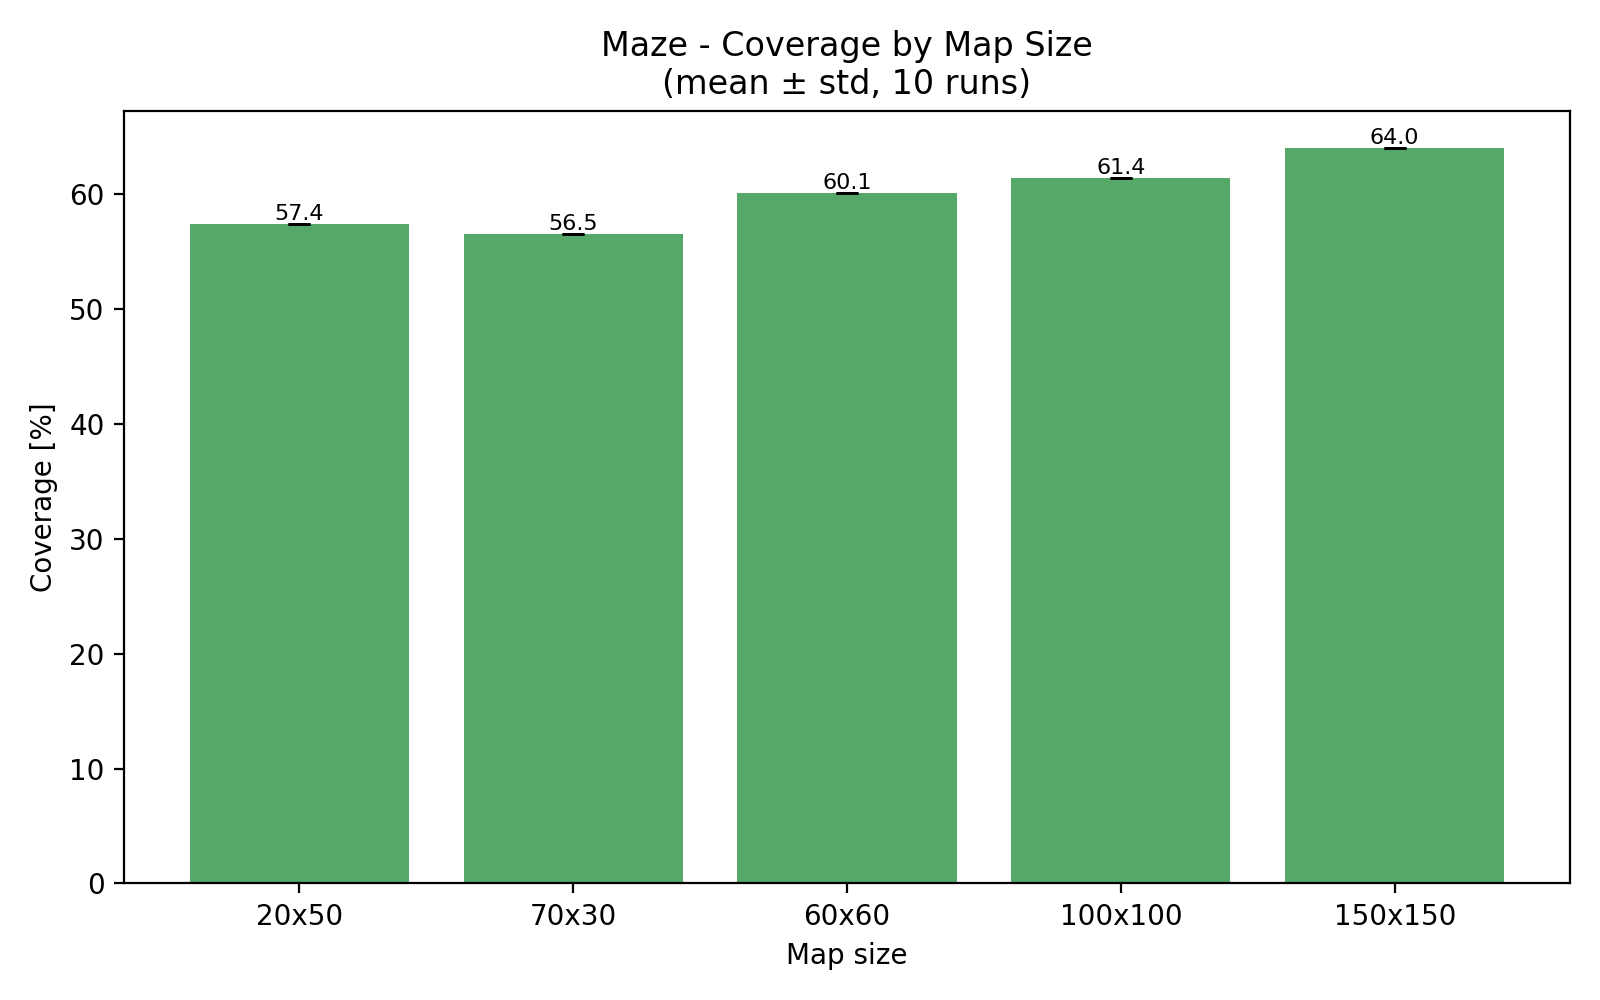
\includegraphics[width=0.75\textwidth]{images/graphs/maze_coverage_by_size.png}
\caption{Bludiště -- průměrné pokrytí podle velikosti mapy}
\label{fig:maze_coverage}
\end{figure}


\subsection{Srovnání algoritmů}

Zobrazené hodnoty jsou průměry přes všechny testované velikosti map, pokud není uvedeno jinak (50 měření na každou kombinaci algoritmu a~velikosti, celkem 250 měření na algoritmus, cyklus proběhl celkem 5$\times$). Konkrétní hodnoty pro jednotlivé velikosti shrnuje tabulka \ref{tab:results_summary}.

\subsubsection{Průměrný čas generování}

Graf \ref{fig:comp_avg_time} zobrazuje průměrný čas generování algoritmů přes všechny testované velikosti map. 
Mezi algoritmy jsou výrazné rozdíly. Nejrychlejšími metodami jsou BSP a~Bludiště, jejichž celkový průměr se pohybuje kolem 7--8 ms. Místnosti dosahují srovnatelného průměru. Náhodná procházka je výrazně pomalejší s~celkovým průměrem přibližně 25 ms. Buněčné automaty jsou řádově nejpomalejší, jejich celkový průměr přesahuje 61 ms, tedy přibližně osmkrát více než u~BSP. 

\begin{figure}[H]
\centering

\includegraphics[width=0.75\textwidth]{images/graphs/comparison_avg_time.png}
\caption{Srovnání průměrného času generování všech algoritmů}
\label{fig:comp_avg_time}
\end{figure}

Na největší testované mapě 150$\times$150 jsou absolutní rozdíly doby generování ještě výraznější: BSP dosahuje 20,3 ms, Bludiště 23,6 ms, Místnosti 26,3 ms, Náhodná procházka 74,1 ms a~Buněčné automaty 178,8 ms (graf \ref{fig:comp_avg_time_150x150}).

\begin{figure}[H]
\centering

\includegraphics[width=0.75\textwidth]{images/graphs/comparison_time_150x150.png}
\caption{Srovnání průměrného času generování na mapě 150$\times$150}
\label{fig:comp_avg_time_150x150}
\end{figure}


\subsubsection{Průměrné pokrytí}

Graf \ref{fig:comp_avg_coverage} zobrazuje průměrné pokrytí mapy průchozím prostorem přes všechny testované velikosti. Nejvyššího celkového pokrytí dosahují Buněčné automaty (přibližně 64 \%), následované algoritmem Bludiště s~pokrytím kolem 60 \%. BSP dosahuje celkového průměru téměř 50 \%, Náhodná procházka má konstrukčně dané pokrytí 50 \%, které se s~velikostí mapy nemění. Místnosti a~chodby dosahují nejnižšího celkového průměru, a~to přibližně 42 \%, avšak pokrytí výrazně roste s~velikostí mapy (viz graf \ref{fig:comp_coverage_scaling}).

\begin{figure}[H]
\centering

\includegraphics[width=0.75\textwidth]{images/graphs/comparison_avg_coverage.png}
\caption{Srovnání průměrného pokrytí všech algoritmů}
\label{fig:comp_avg_coverage}
\end{figure}


\subsubsection{Škálování s velikostí mapy}

Graf \ref{fig:comp_time_scaling} znázorňuje, jak se čas generování mění s~rostoucím počtem buněk mapy. BSP a~Bludiště vykazují přibližně lineární nárůst času. Algoritmus Místností roste rovněž přibližně lineárně, avšak s~vyšší konstantou, protože na velkých mapách generuje výrazně více místností. Náhodná procházka roste rychleji, a~to kvůli opakovanému navracení do již odkrytých oblastí. Buněčné automaty vykazují nejstrmější nárůst.

\begin{figure}[H]
\centering

\includegraphics[width=0.85\textwidth]{images/graphs/comparison_time_scaling.png}
\caption{Škálování času generování s~počtem buněk mapy}
\label{fig:comp_time_scaling}
\end{figure}

Graf \ref{fig:comp_coverage_scaling} ukazuje vývoj pokrytí v~závislosti na velikosti mapy. BSP, Buněčné automaty a~Místnosti vykazují rostoucí tendenci pokrytí s~velikostí mapy. Bludiště má mírně rostoucí, ale velmi stabilní pokrytí. Náhodná procházka zůstává konstantní na hodnotě 50 \%.

Výjimku tvoří mapa 70$\times$30, u~které pokrytí algoritmů Místností, BSP a~Bludiště klesá pod hodnoty dosažené na mapě 20$\times$50, přestože celkový počet buněk je větší (2\,100 vs. 1\,000).

\begin{figure}[H]
\centering

\includegraphics[width=0.85\textwidth]{images/graphs/comparison_coverage_scaling.png}
\caption{Škálování pokrytí s~počtem buněk mapy}
\label{fig:comp_coverage_scaling}
\end{figure}


\subsubsection{Kompromis mezi rychlostí a pokrytím}

Graf \ref{fig:comp_tradeoff} vizualizuje vztah mezi průměrným časem generování a~průměrným pokrytím pro jednotlivé algoritmy (oba průměry přes všechny testované velikosti map). Ideální algoritmus by se nacházel v~levé horní části grafu, tedy s~nízkým časem a~vysokým pokrytím.

BSP a~Bludiště se nacházejí v~oblasti nízkého času a~středně vysokého pokrytí; Bludiště dosahuje vyššího pokrytí (kolem 60 \%) než BSP (kolem 51 \%). Místnosti nabízí srovnatelný čas s~nižším celkovým pokrytím. Buněčné automaty dosahují nejvyššího pokrytí ze všech metod, avšak za cenu výrazně vyššího výpočetního času. Náhodná procházka představuje předvídatelné pokrytí 50 \%, avšak s~vyšším časem generování než BSP, Bludiště a~Místnosti.

\begin{figure}[H]
\centering

\includegraphics[width=0.75\textwidth]{images/graphs/comparison_tradeoff.png}
\caption{Kompromis mezi rychlostí a~pokrytím}
\label{fig:comp_tradeoff}
\end{figure}


\subsubsection{Rozptyl výsledků na velké mapě}

Variabilitu času a~pokrytí na největší testované mapě 150$\times$150 zobrazují boxploty. 

Graf \ref{fig:size150_time_box} ukazuje, že BSP vykazuje nejmenší relativní rozptyl času, zatímco Náhodná procházka má nejvyšší variabilitu. 

\begin{figure}[H]
\centering

\includegraphics[width=0.75\textwidth]{images/graphs/size_150x150_time_boxplot.png}
\caption{Rozptyl času generování na mapě 150$\times$150}
\label{fig:size150_time_box}
\end{figure}

Obrázek \ref{fig:size150_cov_box} ukazuje, že Bludiště a~Náhodná procházka mají prakticky nulovou variabilitu pokrytí, zatímco Místnosti, BSP a~Buněčné automaty vykazují větší rozptyl.

\begin{figure}[H]
\centering

\includegraphics[width=0.75\textwidth]{images/graphs/size_150x150_coverage_boxplot.png}
\caption{Rozptyl pokrytí na mapě 150$\times$150}
\label{fig:size150_cov_box}
\end{figure}


\subsection{Souhrnná tabulka výsledků}

Tabulka \ref{tab:results_summary} obsahuje průměrné hodnoty času generování a~pokrytí mapy pro všechny testované kombinace algoritmů a~velikostí map.

\begin{table}[H]
\centering
\small
\begin{tabular}{|l|r|r|r|r|r|}
\hline
\textbf{Algoritmus} & \textbf{20$\times$50} & \textbf{60$\times$60} & \textbf{70$\times$30} & \textbf{100$\times$100} & \textbf{150$\times$150} \\
\hline
\multicolumn{6}{|c|}{\textit{Průměrný čas generování [ms]}} \\
\hline
Rooms    & 0,88  & 5,59  & 1,46  & 10,01  & 26,33  \\
BSP      & 0,81  & 3,12  & 1,69  & 8,97   & 20,34  \\
Drunkard's  & 3,29  & 10,41 & 6,63  & 30,18  & 74,14  \\
Cellular & 7,10  & 27,60 & 15,47 & 78,34  & 178,83 \\
Maze     & 0,96  & 3,57  & 1,95  & 10,14  & 23,55  \\
\hline
\multicolumn{6}{|c|}{\textit{Průměrné pokrytí [\%]}} \\
\hline
Rooms    & 39,88 & 37,49 & 31,27 & 44,64 & 53,14 \\
BSP      & 46,31 & 50,28 & 44,86 & 52,90 & 53,01 \\
Drunkard's  & 50,06 & 50,02 & 50,03 & 50,01 & 50,00 \\
Cellular & 52,31 & 65,67 & 60,60 & 69,83 & 72,74 \\
Maze     & 57,40 & 60,11 & 56,48 & 61,42 & 64,02 \\
\hline
\end{tabular}
\caption{Průměrný čas generování a~pokrytí}
\label{tab:results_summary}
\end{table}


\subsection{Shrnutí výsledků}

Algoritmy se podle výpočetní náročnosti rozdělují do tří skupin. Do první skupiny patří BSP, Bludiště a~Místnosti, jejichž časy generování na mapě 150$\times$150 nepřekračují 27 ms. Náhodná procházka tvoří střední kategorii s~průměrným časem přibližně 74,1 ms. Buněčné automaty jsou nejpomalejší s~průměrným časem přibližně 178,8 ms.

Z~hlediska pokrytí mapy se algoritmy rovněž výrazně liší. Buněčné automaty dosahují na velkých mapách nejvyššího pokrytí přes 72 \%. Bludiště dosahuje pokrytí v~rozmezí 56--64 \% v~závislosti na velikosti mapy. BSP dosahuje relativně stabilního pokrytí v~rozmezí 45--53 \% napříč všemi velikostmi map. Místnosti dosahují na mapě 150$\times$150 přibližně 53 \%, avšak pokrytí výrazně stoupá s~velikostí mapy (od přibližně 31 \% na mapě 70$\times$30). Náhodná procházka má dané pokrytí 50 \%.

\section{Diskuse}

\subsection{Silné a~slabé stránky jednotlivých metod}

Každý algoritmus vykazuje specifické silné a~slabé stránky, které ovlivňují jeho vhodnost pro různé typy her.

Algoritmus BSP nabízí dobrou rovnováhu mezi rychlostí generování, pokrytím mapy a~strukturovaností výsledku. Generované mapy obsahují jasně oddělené místnosti propojené chodbami. Nevýhodou je poměrně pravidelný vzhled výsledných map.

Algoritmus Místností po úpravě škálování počtu místností dosahuje na velkých mapách výrazně vyššího pokrytí a~zároveň nabízí přirozenější rozložení prostoru. Variabilita mezi běhy je u~tohoto algoritmu vyšší, což zvyšuje znovuhratelnost, ale zároveň snižuje předvídatelnost výsledku.

Buněčné automaty generují přirozeně působící jeskynní struktury, které se nejvíce odlišují od klasického dungeonového prostředí. Dosahují nejvyššího pokrytí ze všech testovaných metod. Hlavní nevýhodou je výrazně vyšší výpočetní náročnost a~možný vznik izolovaných oblastí, které nejsou vzájemně průchozí. Důsledkem těchto izolovaných oblastí je, že výsledné pokrytí zahrnuje i~nepřístupné části mapy. Skutečné přístupné pokrytí je proto nižší, než jakou hodnotu udává měřená metrika.

Náhodná procházka vytváří organicky tvarované chodby s~předvídatelným pokrytím. Konstantní pokrytí může být výhodou v~situacích, kdy je požadována přesná kontrola nad poměrem průchozího prostoru. Nevýhodou je nižší strukturovanost výsledného prostředí.

Implementace algoritmu Bludiště slouží primárně pro demonstraci odlišného přístupu k~procedurálnímu generování. Generuje dokonalé bludiště s~téměř nulovou variabilitou pokrytí a~velmi nízkou variabilitou času. Z~hlediska dungeonových map je však méně vhodný, protože vytváří převážně úzké chodby bez většího otevřeného prostoru.

Naměřené časy generování odpovídají teoretické složitosti jednotlivých algoritmů. Všechny implementované metody dosahují lineární složitosti $O(n)$, kde $n = w \cdot h$; rozdíly v~rychlosti jsou způsobeny konstantními koeficienty. Buněčné automaty provádějí pro každou buňku $s = 5$ průchodů s~vyhodnocením 8~sousedů ($\approx 40 \cdot n$ operací), což vysvětluje přibližně osminásobný časový rozdíl oproti BSP a~Bludiště. Stochastická povaha Náhodné procházky způsobuje opakované navštěvování odkrytých oblastí a~výraznou variabilitu doby generování, i~přes lineární průměrnou složitost. Pokrytí mapy 70$\times$30 klesá u~algoritmů Místností, BSP a~Bludiště pod hodnoty menší mapy 20$\times$50, protože nízký obdélník omezuje rozmístění místností i~použitelné oblasti při dělení mřížky, čímž roste podíl stěn a~okrajů vůči průchoznému prostoru.

\subsection{Zkušenosti z implementace}

U většiny metod zaručoval průchodnost mapy již princip algoritmu -- explicitní propojování místností u~Místností a~BSP, návštěva všech buněk u~Bludiště a~spojitá chůze u~Náhodné procházky. U~Buněčných automatů však mohou po simulaci vzniknout oddělené nepřístupné kapsy. Umísťování hráče je přitom společné pro všechny metody: implementace nejprve pomocí BFS identifikovala největší souvislou oblast podlahových dlaždic a~hráče umístila právě do ní. Jelikož je hráč reprezentován kolizním tělesem o~velikosti $2 \times 2$ dlaždic, umístění vyžadovalo nalezení dlaždice s~volným okolím $3 \times 3$. Pokud taková dlaždice v~největší souvislé oblasti neexistuje, implementace použije záložní pozici $2 \times 2$.

Velikost hráče ovlivnila i~návrh všech generovacích algoritmů. Chodby musely mít šířku alespoň 2 dlaždice, jinak by byla mapa pro hráče neprůchozí. Toto omezení se promítlo například do šířky L-chodeb u~BSP a~Místností, do vykreslování oblastí $2 \times 2$ v~jednotlivých krocích Náhodné procházky a~do velikosti buněk $2 \times 2$ u~algoritmu Bludiště.

Úprava algoritmu Místností, při které pevný počet místností nahradilo škálování úměrné ploše mapy, vedla k~výraznému zlepšení pokrytí na velkých mapách. Další významná úprava proběhla u~BSP, kdy místo fixních 4 průchodů do hloubky algoritmus přešel na rekurzivní dělení, které pokračuje, dokud by výsledné podoblasti nebyly menší než \texttt{MIN\_SIZE~$\times$~2}.

Ladění parametrů Buněčných automatů, konkrétně počtu simulačních kroků, mělo značný dopad na výsledek. Při 3 krocích zůstávaly v~mapě četné izolované buňky, při 10 krocích se struktury výrazně vyhladily a~pokrytí vzrostlo, avšak za cenu vyššího výpočetního času a~velkého prázdného prostoru bez struktury. Hodnota 5 kroků představuje kompromis mezi kvalitou výsledných struktur a~časovou náročností. Podobně parametr \texttt{TARGET\_COVERAGE} u~Náhodné procházky přímo určuje podíl průchozího prostoru, vyšší hodnota prodlužovala dobu generování a~struktura byla opět velmi souvislá.

I~drobná změna parametrizace může zásadně ovlivnit výsledné vlastnosti generovaného prostředí, jeho pokrytí, strukturu i~čas generování.

\subsection{Souvislost s předchozím výzkumem}

Práce \cite{Monaghan2019} rovněž porovnávala efektivitu PCG algoritmů pro generování 2D map a~měřila čas generování a~spotřebu výpočetních zdrojů kombinací algoritmů pro umísťování místností (Random Room Placement, BSP) a~propojování chodbami (Random Point Connect, Drunkard's Walk, BSP Corridors). Oproti tomuto přístupu se předkládaná práce zaměřuje na pět samostatných generovacích metod (včetně Buněčných automatů a~generování Bludiště) a~jako metriku používá vedle času generování také pokrytí mapy průchozím prostorem. Obě práce se však shodují v~závěru, že BSP patří mezi nejefektivnější přístupy z~hlediska času generování.

\subsection{Možnosti dalšího rozšíření práce}
Prvním směrem rozšíření je zahrnutí strukturálních metrik. Pokrytí mapy průchozím prostorem je snadno měřitelná a~objektivní metrika, avšak sama o~sobě nevypovídá o~strukturální kvalitě generovaného prostředí. Dvě mapy se stejným pokrytím se mohou zásadně lišit z~hlediska hratelnosti. Například Bludiště a~Buněčné automaty dosahují na mapě 60$\times$60 podobného pokrytí (přibližně 60 a~66 \%), přesto jsou výsledné struktury zcela odlišné: Bludiště vytváří spletitou síť úzkých chodeb, zatímco Buněčné automaty generují otevřené jeskynní prostory.

Relevantnějšími doplňkovými metrikami by mohly být například průměrná délka nejkratší cesty mezi dvěma náhodně vybranými průchozími dlaždicemi (měřitelná pomocí BFS), podíl slepých uliček nebo průměrný počet prostorově oddělených místností. Tyto metriky by umožnily kvantitativně zachytit rozdíly, které se v~současném měření projevují pouze vizuálně, a~lépe posoudit vhodnost jednotlivých metod pro konkrétní typy herního prostředí.

Dalším směrem je kombinace více metod v~jedné mapě, například vyplnění BSP místností buněčnými automaty pro dosažení přirozenějšího vzhledu.
Užitečným rozšířením by bylo také přidání sémantických pravidel pro rozmístění herních prvků, například zajištění, aby klíčové předměty ležely v~dostatečné vzdálenosti od startu hráče, nebo adaptivní generování přizpůsobující parametry algoritmů postupu hráče hrou.

%% Závěry práce
\begin{kiconclusions}
Práce implementovala a~experimentálně porovnala pět algoritmů procedurálního generování dungeonových map ve 2D hrách v~herním enginu Godot.

V~teoretické části práce popsala základní principy procedurálního generování obsahu, jeho historický vývoj a~přehled vybraných metod včetně jejich výhod a~omezení. Z~rešeršní části práce vybrala pět algoritmů reprezentujících různé přístupy ke generování map: Náhodné umístění místností a~chodeb, Binary Space Partitioning, Náhodná procházka (Drunkard's Walk), Buněčné automaty a~generování Bludiště.

Práce implementovala všech pět algoritmů v~herním enginu Godot s~využitím skriptovacího jazyka GDScript. Systém vznikl v~modulárním návrhu s~unifikovaným rozhraním, které umožňuje snadné přidávání nových generovacích metod. Součástí aplikace je automatizovaný benchmarkový režim, který zajišťuje objektivní a~opakovatelné měření výkonu jednotlivých algoritmů.

Experimentální měření proběhlo na pěti velikostech map v~deseti nezávislých bězích pro každou konfiguraci, a~to celkem 5$\times$. Výsledky ukázaly výrazné rozdíly mezi metodami. Algoritmy BSP a~Bludiště se ukázaly jako nejrychlejší s~časy kolem 20--24 ms na mapě 150$\times$150. Algoritmus Místností dosahuje pokrytí přibližně 53 \% na největší mapě. Buněčné automaty generují mapy s~nejvyšším pokrytím (přes 72 \%), avšak s~výrazně vyšším výpočetním časem, a~to přibližně 178,8 ms na mapě 150$\times$150. Náhodná procházka poskytuje konstrukčně dané pokrytí 50 \%, avšak s~vyšším časem generování, přibližně 74 ms na největší mapě.

Práce ukázala, že volba generovací metody závisí na konkrétních požadavcích hry, protože každá metoda vytváří odlišný typ prostředí. Pro klasické dungeonové prostředí jsou vhodné algoritmy BSP a~Místnosti, pro jeskynní struktury jsou ideální Buněčné automaty a~Náhodná procházka a~pro labyrinty algoritmus Bludiště.

Mezi hlavní omezení práce patří testování výhradně v~prostředí Godot s~jazykem GDScript a~měření na jednom hardwarovém zařízení (MacBook Air 2025, M4, 24~GB RAM). Benchmarkové měření probíhalo bez fixovaného seedu, takže individuální výsledky konkrétního běhu nelze přesně reprodukovat. Statistické závěry jsou však podloženy 50~měřeními na každou konfiguraci.
\end{kiconclusions}

\begin{kiconclusions}[english]
This thesis implemented and experimentally compared five algorithms for procedural dungeon map generation in 2D games in the Godot game engine.

The theoretical part described the basic principles of procedural content generation, its historical development, and an overview of selected methods, including their advantages and limitations. From the literature review, the thesis selected five algorithms representing different approaches to map generation: Random room placement, Binary Space Partitioning, Drunkard's walk, Cellular automata, and Maze generation.

All five algorithms were implemented in the Godot game engine using the GDScript scripting language. The system uses a~modular design with a~unified interface that allows easy addition of new generation methods. The application includes an automated benchmark mode that ensures objective and repeatable performance measurements.

Experimental measurements were conducted on five map sizes with ten independent runs per configuration, repeated five times in total. The results showed significant differences between the methods. BSP and Maze proved to be the fastest algorithms, with generation times around 20--24 ms on a~150$\times$150 map. The Rooms algorithm achieves approximately 53 \% coverage on the largest map. Cellular automata generate maps with the highest coverage (over 72 \%), but at the cost of significantly higher computation time of approximately 178.8 ms on a~150$\times$150 map. Drunkard's walk provides a~structurally fixed coverage of 50 \%, but with a~higher generation time of approximately 74 ms on the largest map.

The choice of generation method depends on the specific requirements of the game: BSP and Rooms are suitable for classic dungeon environments, cellular automata and drunkard's walk for cave-like structures, and the Maze algorithm for labyrinthine layouts.

Limitations of this work include testing exclusively in the Godot environment with GDScript and measurements on a~single hardware device (MacBook Air 2025, M4, 24~GB RAM). The benchmark measurements were conducted without a fixed random seed, meaning individual run results cannot be precisely reproduced; however, the statistical conclusions are supported by 50 measurements per configuration.
\end{kiconclusions}

%% Přílohy
\appendix

\section{Odkaz na repozitář projektu}

Zdrojový kód aplikace je dostupný v~repozitáři na platformě GitHub:

\begin{center}
\url{https://github.com/Jim-23/ProceduralGenerationBP}
\end{center}

\section{Zkratky}
\begin{description}
\item[2D] Two-Dimensional
\item[3D] Three-Dimensional
\item[ASCII] American Standard Code for Information Interchange
\item[BBC Micro] British Broadcasting Corporation Microcomputer
\item[BFS] Breadth-first search
\item[BSP] Binary Space Partitioning
\item[CSV] Comma-Separated Values
\item[DFS] Depth-First Search
\item[PCG] Procedural Content Generation
\item[RAM] Random Access Memory
\end{description}

%% Obsah elektronických dat.
\section{Obsah elektronických dat} \label{sec:ObsahData}

Elektronická data práce tvoří ZIP archiv celého projektu s~následující strukturou:

\begin{description}

\item[\texttt{src/}] \hfill \\
  Zdrojové soubory projektu a~\texttt{README.txt} s~instrukcemi pro spuštění aplikace.

\item[\texttt{text/}] \hfill \\
  Adresář s~textem bakalářské práce.

\end{description}

%% -------------------------------------------------------------------

%% Sazba volitelného seznamu zkratek, za přílohami.
%%printglossary

%% Sazba povinné bibliografie, za přílohami (případně i za seznamem
%% zkratek). Při použití BibLaTeXu použijte makro
%% \printbibliography. jinak prostředí thebibliography. Ne obojí!

%% Vlastní sazba bibliografie při použití BibLaTeXu.
\printbibliography

%% Bibliografie, včetně sazby, při NEpoužití BibLaTeXu.
% \begin{thebibliography}{9}
%\bibitem{kniha2} \uppercase{Hawke}, Paul. NanoHttpd: Light-weight HTTP server designed for embedding in other applications. GitHub [online]. 2014-05-12. [cit. 2014-12-06]. Dostupné z: \url{https://github.com/NanoHttpd/nanohttpd}
%
%\bibitem{jeske13} \uppercase{Jeske}, David; \uppercase{Novák}, Josef. Simple HTTP Server in \csharp: Threaded synchronous HTTP Server abstract class, to respond to HTTP requests. CodeProject: For those who code [online]. 2014-05-24. [cit. 2014-12-06]. Dostupné z: \url{http://www.codeproject.com/Articles/137979/Simple-HTTP-Server-in-C}
%
%\bibitem{uzis2012} \uppercase{ÚSTAV ZDRAVOTNICKÝCH INFORMACÍ A STATISTIKY ČR}. Lékaři, zubní lékaři a farmaceuti 2012 [online]. Praha 2, Palackého náměstí 4: Ústav zdravotnických informací a statistiky ČR, 2012 [cit. 2014-12-06]. ISBN 978-80-7472-089-5. Dostupné z: \url{http://www.uzis.cz/publikace/lekari-zubni-lekari-farmaceuti-2012}
% \end{thebibliography}

%% Sazba volitelného rejstříku, za bibliografií.
\printindex

\end{document}

%%% Local Variables:
%%% mode: latex
%%% TeX-master: t
%%% End:
